\hypertarget{_lgm___date_and_time_8c}{
\section{/home/mgh/LanlGeoMag/libLanlGeoMag/Lgm\_\-DateAndTime.c File Reference}
\label{_lgm___date_and_time_8c}\index{/home/mgh/LanlGeoMag/libLanlGeoMag/Lgm\_\-DateAndTime.c@{/home/mgh/LanlGeoMag/libLanlGeoMag/Lgm\_\-DateAndTime.c}}
}
{\tt \#include $<$stdio.h$>$}\par
{\tt \#include $<$stdlib.h$>$}\par
{\tt \#include $<$math.h$>$}\par
{\tt \#include \char`\"{}Lgm/Lgm\_\-CTrans.h\char`\"{}}\par


Include dependency graph for Lgm\_\-DateAndTime.c:\nopagebreak
\begin{figure}[H]
\begin{center}
\leavevmode
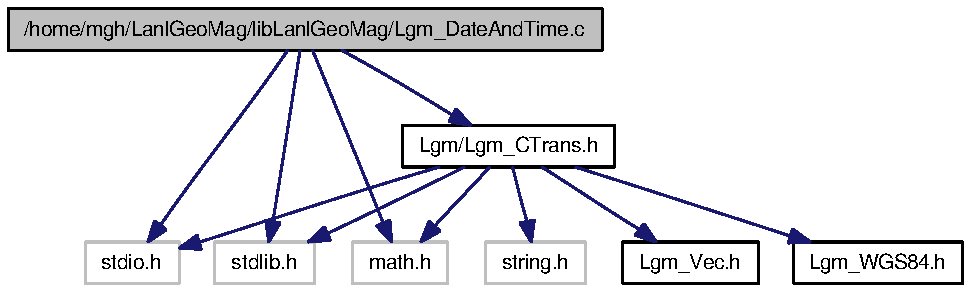
\includegraphics[width=250pt]{_lgm___date_and_time_8c__incl}
\end{center}
\end{figure}
\subsection*{Functions}
\begin{CompactItemize}
\item 
int \hyperlink{_lgm___date_and_time_8c_5b729962975e5532cb9d9a3edf09d73e}{Lgm\_\-LeapYear} (int year)
\item 
double \hyperlink{_lgm___date_and_time_8c_de46e5122248c7bf19ce56f2ed4b7e91}{Lgm\_\-GetLeapSeconds} (double JD, \hyperlink{struct_lgm___c_trans}{Lgm\_\-CTrans} $\ast$c)
\item 
int \hyperlink{_lgm___date_and_time_8c_7d638a5de1c5a2b0176e2c51f4e85427}{Lgm\_\-IsLeapSecondDay} (long int Date, double $\ast$SecondsInDay, \hyperlink{struct_lgm___c_trans}{Lgm\_\-CTrans} $\ast$c)
\item 
int \hyperlink{_lgm___date_and_time_8c_ffe919b2830c07067e255ca1a454a05a}{Lgm\_\-LoadLeapSeconds} (\hyperlink{struct_lgm___c_trans}{Lgm\_\-CTrans} $\ast$c)
\item 
void \hyperlink{_lgm___date_and_time_8c_38a6c5c43a1767d6f26c90f7970882e0}{Lgm\_\-TAI\_\-to\_\-GPS} (\hyperlink{struct_lgm___date_time}{Lgm\_\-DateTime} $\ast$TAI, \hyperlink{struct_lgm___date_time}{Lgm\_\-DateTime} $\ast$GPS, \hyperlink{struct_lgm___c_trans}{Lgm\_\-CTrans} $\ast$c)
\item 
void \hyperlink{_lgm___date_and_time_8c_ae7db2b4a40466c781a6a29f91a51133}{Lgm\_\-GPS\_\-to\_\-TAI} (\hyperlink{struct_lgm___date_time}{Lgm\_\-DateTime} $\ast$GPS, \hyperlink{struct_lgm___date_time}{Lgm\_\-DateTime} $\ast$TAI, \hyperlink{struct_lgm___c_trans}{Lgm\_\-CTrans} $\ast$c)
\item 
void \hyperlink{_lgm___date_and_time_8c_ab03f400cbc08ffa12348eb15bf37eb5}{Lgm\_\-UTC\_\-to\_\-GPS} (\hyperlink{struct_lgm___date_time}{Lgm\_\-DateTime} $\ast$UTC, \hyperlink{struct_lgm___date_time}{Lgm\_\-DateTime} $\ast$GPS, \hyperlink{struct_lgm___c_trans}{Lgm\_\-CTrans} $\ast$c)
\item 
void \hyperlink{_lgm___date_and_time_8c_1ff96bc78656dfc6ab411f6b4d8993f1}{Lgm\_\-GPS\_\-to\_\-UTC} (\hyperlink{struct_lgm___date_time}{Lgm\_\-DateTime} $\ast$GPS, \hyperlink{struct_lgm___date_time}{Lgm\_\-DateTime} $\ast$UTC, \hyperlink{struct_lgm___c_trans}{Lgm\_\-CTrans} $\ast$c)
\item 
double \hyperlink{_lgm___date_and_time_8c_62bc389169141b90c128c1413f10ba9a}{Lgm\_\-GPS\_\-to\_\-GpsSeconds} (\hyperlink{struct_lgm___date_time}{Lgm\_\-DateTime} $\ast$GPS)
\item 
void \hyperlink{_lgm___date_and_time_8c_2170efd02fc5e37005be974bf1688753}{Lgm\_\-GpsSeconds\_\-to\_\-GPS} (double GpsSeconds, \hyperlink{struct_lgm___date_time}{Lgm\_\-DateTime} $\ast$GPS)
\item 
void \hyperlink{_lgm___date_and_time_8c_e359f512f21bf55270e5454b9089cf2f}{Lgm\_\-GpsSeconds\_\-to\_\-UTC} (double GpsSeconds, \hyperlink{struct_lgm___date_time}{Lgm\_\-DateTime} $\ast$UTC, \hyperlink{struct_lgm___c_trans}{Lgm\_\-CTrans} $\ast$c)
\item 
double \hyperlink{_lgm___date_and_time_8c_a242e28151e439aefeb83cd85c735903}{Lgm\_\-UTC\_\-to\_\-GpsSeconds} (\hyperlink{struct_lgm___date_time}{Lgm\_\-DateTime} $\ast$UTC, \hyperlink{struct_lgm___c_trans}{Lgm\_\-CTrans} $\ast$c)
\item 
double \hyperlink{_lgm___date_and_time_8c_8d1a12a1442f0fed2e64749c47db8157}{Lgm\_\-TAI\_\-to\_\-TaiSeconds} (\hyperlink{struct_lgm___date_time}{Lgm\_\-DateTime} $\ast$TAI)
\item 
void \hyperlink{_lgm___date_and_time_8c_39c239611e99c1ad3a2ae8af2cb93d9c}{Lgm\_\-TaiSeconds\_\-to\_\-TAI} (double TaiSeconds, \hyperlink{struct_lgm___date_time}{Lgm\_\-DateTime} $\ast$TAI)
\item 
void \hyperlink{_lgm___date_and_time_8c_906b9059ecb4e21fa8bf26b91df3dbad}{Lgm\_\-TaiSeconds\_\-to\_\-UTC} (double TaiSeconds, \hyperlink{struct_lgm___date_time}{Lgm\_\-DateTime} $\ast$UTC, \hyperlink{struct_lgm___c_trans}{Lgm\_\-CTrans} $\ast$c)
\item 
double \hyperlink{_lgm___date_and_time_8c_9c99186b444f75dd856bd789298b9cb8}{Lgm\_\-UTC\_\-to\_\-TaiSeconds} (\hyperlink{struct_lgm___date_time}{Lgm\_\-DateTime} $\ast$UTC, \hyperlink{struct_lgm___c_trans}{Lgm\_\-CTrans} $\ast$c)
\item 
void \hyperlink{_lgm___date_and_time_8c_fc2358593ed2c075d04b1ae6663a86a6}{Lgm\_\-UTC\_\-to\_\-TAI} (\hyperlink{struct_lgm___date_time}{Lgm\_\-DateTime} $\ast$UTC, \hyperlink{struct_lgm___date_time}{Lgm\_\-DateTime} $\ast$TAI, \hyperlink{struct_lgm___c_trans}{Lgm\_\-CTrans} $\ast$c)
\item 
void \hyperlink{_lgm___date_and_time_8c_de5bfe94202a0503dbbe1cb6a066ecf9}{Lgm\_\-TAI\_\-to\_\-UTC} (\hyperlink{struct_lgm___date_time}{Lgm\_\-DateTime} $\ast$TAI, \hyperlink{struct_lgm___date_time}{Lgm\_\-DateTime} $\ast$UTC, \hyperlink{struct_lgm___c_trans}{Lgm\_\-CTrans} $\ast$c)
\item 
void \hyperlink{_lgm___date_and_time_8c_1c9dffe866b03fe6c519bba85445b8ef}{Lgm\_\-TT\_\-to\_\-TAI} (\hyperlink{struct_lgm___date_time}{Lgm\_\-DateTime} $\ast$TT, \hyperlink{struct_lgm___date_time}{Lgm\_\-DateTime} $\ast$TAI, \hyperlink{struct_lgm___c_trans}{Lgm\_\-CTrans} $\ast$c)
\item 
void \hyperlink{_lgm___date_and_time_8c_df975a9192e9f08e25898ad3bdf906ff}{Lgm\_\-TAI\_\-to\_\-TT} (\hyperlink{struct_lgm___date_time}{Lgm\_\-DateTime} $\ast$TAI, \hyperlink{struct_lgm___date_time}{Lgm\_\-DateTime} $\ast$TT, \hyperlink{struct_lgm___c_trans}{Lgm\_\-CTrans} $\ast$c)
\item 
void \hyperlink{_lgm___date_and_time_8c_22d70f08569629bfb06991502e8a2943}{Lgm\_\-TT\_\-to\_\-TDB} (\hyperlink{struct_lgm___date_time}{Lgm\_\-DateTime} $\ast$TT, \hyperlink{struct_lgm___date_time}{Lgm\_\-DateTime} $\ast$TDB, \hyperlink{struct_lgm___c_trans}{Lgm\_\-CTrans} $\ast$c)
\item 
void \hyperlink{_lgm___date_and_time_8c_10a71e0d594a09fd5a859d481a7c9dc6}{Lgm\_\-TT\_\-to\_\-TDB\_\-IAU2006} (\hyperlink{struct_lgm___date_time}{Lgm\_\-DateTime} $\ast$TT, \hyperlink{struct_lgm___date_time}{Lgm\_\-DateTime} $\ast$TDB, \hyperlink{struct_lgm___c_trans}{Lgm\_\-CTrans} $\ast$c)
\item 
void \hyperlink{_lgm___date_and_time_8c_0d5b5fb558ccb33fe27b2a5452c8e143}{Lgm\_\-TDB\_\-to\_\-TT} (\hyperlink{struct_lgm___date_time}{Lgm\_\-DateTime} $\ast$TDB, \hyperlink{struct_lgm___date_time}{Lgm\_\-DateTime} $\ast$TT, \hyperlink{struct_lgm___c_trans}{Lgm\_\-CTrans} $\ast$c)
\item 
void \hyperlink{_lgm___date_and_time_8c_5ee50179c8f841ba7e3377fc23793c37}{Lgm\_\-UTC\_\-to\_\-TT} (\hyperlink{struct_lgm___date_time}{Lgm\_\-DateTime} $\ast$UTC, \hyperlink{struct_lgm___date_time}{Lgm\_\-DateTime} $\ast$TT, \hyperlink{struct_lgm___c_trans}{Lgm\_\-CTrans} $\ast$c)
\item 
void \hyperlink{_lgm___date_and_time_8c_a574b2bf1ef2d8826ecda810565ffc78}{Lgm\_\-TT\_\-to\_\-UTC} (\hyperlink{struct_lgm___date_time}{Lgm\_\-DateTime} $\ast$TT, \hyperlink{struct_lgm___date_time}{Lgm\_\-DateTime} $\ast$UTC, \hyperlink{struct_lgm___c_trans}{Lgm\_\-CTrans} $\ast$c)
\item 
void \hyperlink{_lgm___date_and_time_8c_f30246cdf6676c764baedf2ee8717e9b}{Lgm\_\-UTC\_\-to\_\-TDB} (\hyperlink{struct_lgm___date_time}{Lgm\_\-DateTime} $\ast$UTC, \hyperlink{struct_lgm___date_time}{Lgm\_\-DateTime} $\ast$TDB, \hyperlink{struct_lgm___c_trans}{Lgm\_\-CTrans} $\ast$c)
\item 
void \hyperlink{_lgm___date_and_time_8c_04a7c2b17ac1343bdb83bdc8d2204719}{Lgm\_\-TDB\_\-to\_\-UTC} (\hyperlink{struct_lgm___date_time}{Lgm\_\-DateTime} $\ast$TDB, \hyperlink{struct_lgm___date_time}{Lgm\_\-DateTime} $\ast$UTC, \hyperlink{struct_lgm___c_trans}{Lgm\_\-CTrans} $\ast$c)
\item 
\hyperlink{struct_lgm___date_time}{Lgm\_\-DateTime} $\ast$ \hyperlink{_lgm___date_and_time_8c_f1fcad21e7b32777e138bb09ca9f8120}{Lgm\_\-DateTime\_\-Create} (int Year, int Month, int Day, double Time, int TimeSystem, \hyperlink{struct_lgm___c_trans}{Lgm\_\-CTrans} $\ast$c)
\item 
int \hyperlink{_lgm___date_and_time_8c_108f442f417d37e973701a8fae629ba9}{Lgm\_\-Make\_\-UTC} (long int Date, double Time, \hyperlink{struct_lgm___date_time}{Lgm\_\-DateTime} $\ast$UTC, \hyperlink{struct_lgm___c_trans}{Lgm\_\-CTrans} $\ast$c)
\item 
void \hyperlink{_lgm___date_and_time_8c_595e9eed10d25d2eb715e7554e83d3f7}{Lgm\_\-Print\_\-DateTime} (\hyperlink{struct_lgm___date_time}{Lgm\_\-DateTime} DT, int Style, int p)
\item 
void \hyperlink{_lgm___date_and_time_8c_2ec916c82548955c3534f4605ea18c93}{Lgm\_\-DateTimeToString} (char $\ast$Str, \hyperlink{struct_lgm___date_time}{Lgm\_\-DateTime} DT, int Style, int p)
\item 
void \hyperlink{_lgm___date_and_time_8c_950485658fca76d3318ee667798563c4}{Lgm\_\-Print\_\-SimpleTime} (\hyperlink{struct_lgm___date_time}{Lgm\_\-DateTime} $\ast$DT, int p, char $\ast$Str)
\item 
double \hyperlink{_lgm___date_and_time_8c_73a444d73b7a1119517c60f5a070cc9d}{Lgm\_\-JD} (int Year, int Month, int Day, double Time, int TimeSystem, \hyperlink{struct_lgm___c_trans}{Lgm\_\-CTrans} $\ast$c)
\item 
long int \hyperlink{_lgm___date_and_time_8c_e869fd88ef397bce460b886a6a1b840d}{Lgm\_\-JDN} (int Year, int Month, int Day)
\item 
double \hyperlink{_lgm___date_and_time_8c_43cca8555131bec5ffeb9d6d39c34b9b}{Lgm\_\-MJD} (int ny, int nm, int nd, double UT, int TimeSystem, \hyperlink{struct_lgm___c_trans}{Lgm\_\-CTrans} $\ast$c)
\item 
double \hyperlink{_lgm___date_and_time_8c_ceea9bbfdf0bc68de7a2fe4e406707a3}{Lgm\_\-Date\_\-to\_\-JD} (long int Date, double UT, \hyperlink{struct_lgm___c_trans}{Lgm\_\-CTrans} $\ast$c)
\item 
int \hyperlink{_lgm___date_and_time_8c_1808acdcc963d25827db876e77d17b5f}{Lgm\_\-DayOfYear} (int year, int month, int day, \hyperlink{struct_lgm___c_trans}{Lgm\_\-CTrans} $\ast$c)
\item 
int \hyperlink{_lgm___date_and_time_8c_38f91ae9f05bbcd134091cea464ee003}{Lgm\_\-DayOfWeek} (int Year, int Month, int Day, char $\ast$dowstr)
\item 
int \hyperlink{_lgm___date_and_time_8c_55fe73d488049143abdf53aed109af07}{Lgm\_\-Doy} (long int date, int $\ast$YY, int $\ast$MM, int $\ast$DD, int $\ast$DOY)
\item 
int \hyperlink{_lgm___date_and_time_8c_b9dde7da7103f227bc6b698bed55e9ab}{Lgm\_\-IsValidDate} (long int Date)
\item 
double \hyperlink{_lgm___date_and_time_8c_af81b2f637efd027fd4fb425f16dd027}{Lgm\_\-RemapTime} (double Time, double SecondsInADay)
\item 
double \hyperlink{_lgm___date_and_time_8c_70d002da98009a23c04a5ba8a934caeb}{Lgm\_\-UTC\_\-to\_\-TDBSeconds} (\hyperlink{struct_lgm___date_time}{Lgm\_\-DateTime} $\ast$UTC, \hyperlink{struct_lgm___c_trans}{Lgm\_\-CTrans} $\ast$c)
\item 
double \hyperlink{_lgm___date_and_time_8c_07aa79aa96c76993e5770b7a5967f663}{Lgm\_\-TDBSecSinceJ2000} (\hyperlink{struct_lgm___date_time}{Lgm\_\-DateTime} $\ast$UTC, \hyperlink{struct_lgm___c_trans}{Lgm\_\-CTrans} $\ast$c)
\end{CompactItemize}


\subsection{Function Documentation}
\hypertarget{_lgm___date_and_time_8c_5b729962975e5532cb9d9a3edf09d73e}{
\index{Lgm\_\-DateAndTime.c@{Lgm\_\-DateAndTime.c}!Lgm\_\-LeapYear@{Lgm\_\-LeapYear}}
\index{Lgm\_\-LeapYear@{Lgm\_\-LeapYear}!Lgm_DateAndTime.c@{Lgm\_\-DateAndTime.c}}
\subsubsection[{Lgm\_\-LeapYear}]{\setlength{\rightskip}{0pt plus 5cm}int Lgm\_\-LeapYear (int {\em year})}}
\label{_lgm___date_and_time_8c_5b729962975e5532cb9d9a3edf09d73e}




Definition at line 16 of file Lgm\_\-DateAndTime.c.

Here is the caller graph for this function:\nopagebreak
\begin{figure}[H]
\begin{center}
\leavevmode
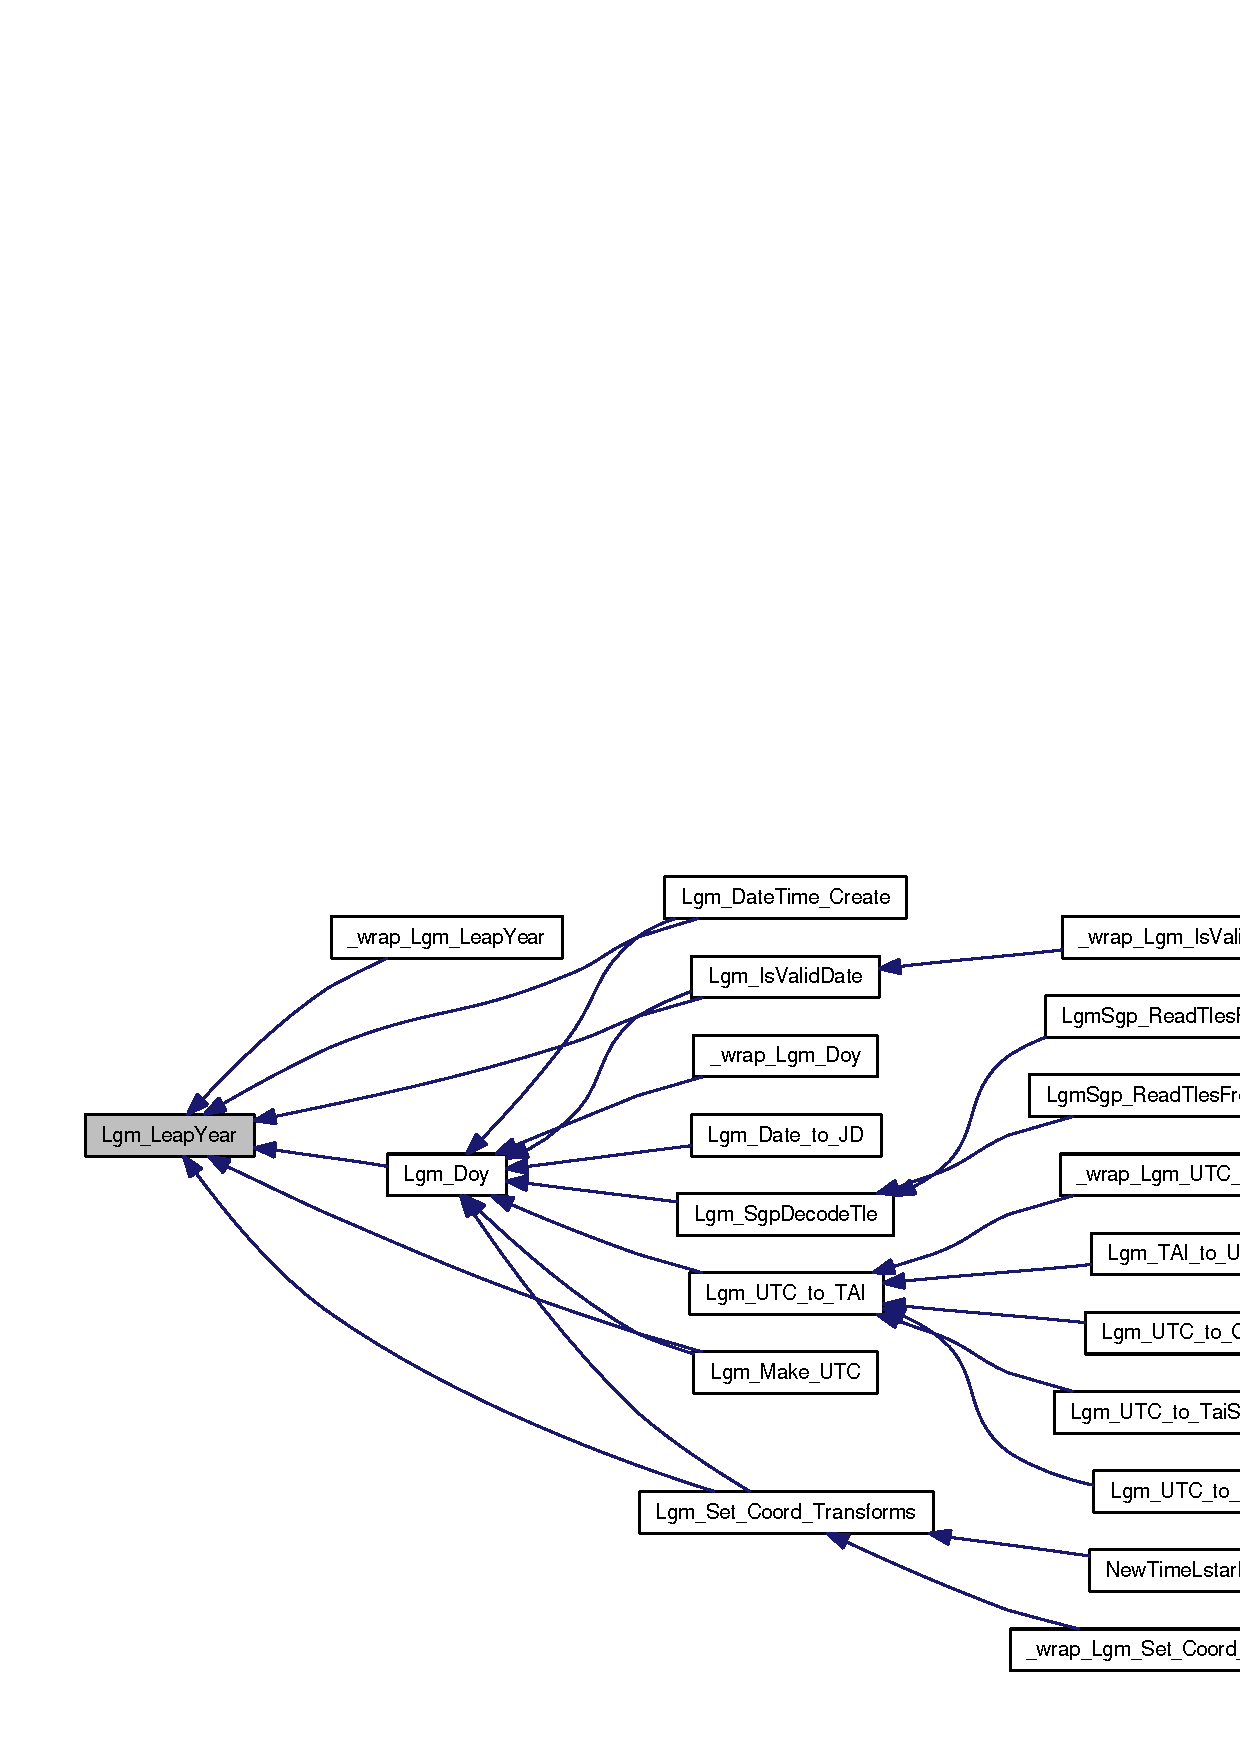
\includegraphics[width=420pt]{_lgm___date_and_time_8c_5b729962975e5532cb9d9a3edf09d73e_icgraph}
\end{center}
\end{figure}
\hypertarget{_lgm___date_and_time_8c_de46e5122248c7bf19ce56f2ed4b7e91}{
\index{Lgm\_\-DateAndTime.c@{Lgm\_\-DateAndTime.c}!Lgm\_\-GetLeapSeconds@{Lgm\_\-GetLeapSeconds}}
\index{Lgm\_\-GetLeapSeconds@{Lgm\_\-GetLeapSeconds}!Lgm_DateAndTime.c@{Lgm\_\-DateAndTime.c}}
\subsubsection[{Lgm\_\-GetLeapSeconds}]{\setlength{\rightskip}{0pt plus 5cm}double Lgm\_\-GetLeapSeconds (double {\em JD}, \/  {\bf Lgm\_\-CTrans} $\ast$ {\em c})}}
\label{_lgm___date_and_time_8c_de46e5122248c7bf19ce56f2ed4b7e91}


Routines for dealing with leap seconds. Also time conversions that require knowledge about leap seconds.

\hyperlink{_lgm___c_trans_8h_de46e5122248c7bf19ce56f2ed4b7e91}{Lgm\_\-GetLeapSeconds()} \hyperlink{_lgm___c_trans_8h_7d638a5de1c5a2b0176e2c51f4e85427}{Lgm\_\-IsLeapSecondDay()} \hyperlink{_lgm___c_trans_8h_ffe919b2830c07067e255ca1a454a05a}{Lgm\_\-LoadLeapSeconds()}

Leap seconds are added when necessary. First preference is given to opportunities at the end of December and the end of June. However, secondary preference is also given to opportunities at the end of March and September if needed. Since leap seconds were introduced in 1972, only dates in December and June have been used to include leap seconds.

Needed to convert between TT or TAI, TDB and UTC. Some defs:

JD -- Julian Date MJD -- Modified Julian Date (JD - 2400000.5) UT -- Universal Time (before 1960 astro calcs were done with UT) ET -- Ephermeris Time (then ET replaced it) TDT -- Terrestrial Dynamical Time (TDT replaced ET in 1981) TT -- Terrestrial Time (in 1991 TDT was renamed to be TT) UTC -- Universal Time Coordinated TAI -- International Atomic Time TDB -- Terrestrial Barycentric Time UT1 -- Universal Time (UT1 is a corrected version of UT0) UT0 -- Universal Time (not used in this uncorrected form) dT -- different between TT and UT1 (i.e. dT = TT-UT1) (this was 32.184s when TAI was introduced in 1958 -- hence the definitions below).

Related by:

TAI = UTC + dAT TT = TAI + 32.184 (i.e. TT = UTC + dAT + 32.184 )

This routine simply determined what the dAT value should be for a given JD. Note that after 1972 they are just leap seconds, but before they are non-integral (leap seconds (werent invented yet?) 

Definition at line 70 of file Lgm\_\-DateAndTime.c.

Here is the caller graph for this function:\nopagebreak
\begin{figure}[H]
\begin{center}
\leavevmode
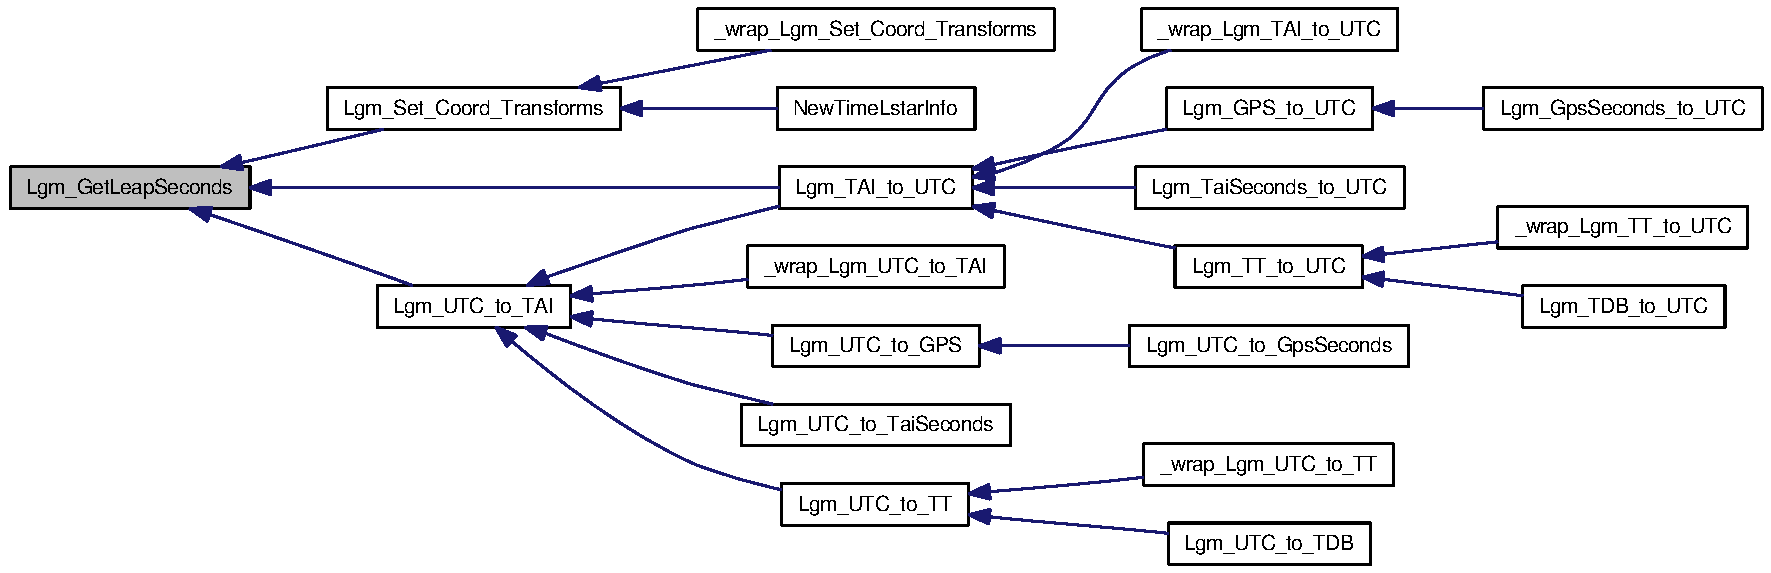
\includegraphics[width=420pt]{_lgm___date_and_time_8c_de46e5122248c7bf19ce56f2ed4b7e91_icgraph}
\end{center}
\end{figure}
\hypertarget{_lgm___date_and_time_8c_7d638a5de1c5a2b0176e2c51f4e85427}{
\index{Lgm\_\-DateAndTime.c@{Lgm\_\-DateAndTime.c}!Lgm\_\-IsLeapSecondDay@{Lgm\_\-IsLeapSecondDay}}
\index{Lgm\_\-IsLeapSecondDay@{Lgm\_\-IsLeapSecondDay}!Lgm_DateAndTime.c@{Lgm\_\-DateAndTime.c}}
\subsubsection[{Lgm\_\-IsLeapSecondDay}]{\setlength{\rightskip}{0pt plus 5cm}int Lgm\_\-IsLeapSecondDay (long int {\em Date}, \/  double $\ast$ {\em SecondsInDay}, \/  {\bf Lgm\_\-CTrans} $\ast$ {\em c})}}
\label{_lgm___date_and_time_8c_7d638a5de1c5a2b0176e2c51f4e85427}




Definition at line 121 of file Lgm\_\-DateAndTime.c.

Here is the caller graph for this function:\nopagebreak
\begin{figure}[H]
\begin{center}
\leavevmode
\includegraphics[width=420pt]{_lgm___date_and_time_8c_7d638a5de1c5a2b0176e2c51f4e85427_icgraph}
\end{center}
\end{figure}
\hypertarget{_lgm___date_and_time_8c_ffe919b2830c07067e255ca1a454a05a}{
\index{Lgm\_\-DateAndTime.c@{Lgm\_\-DateAndTime.c}!Lgm\_\-LoadLeapSeconds@{Lgm\_\-LoadLeapSeconds}}
\index{Lgm\_\-LoadLeapSeconds@{Lgm\_\-LoadLeapSeconds}!Lgm_DateAndTime.c@{Lgm\_\-DateAndTime.c}}
\subsubsection[{Lgm\_\-LoadLeapSeconds}]{\setlength{\rightskip}{0pt plus 5cm}int Lgm\_\-LoadLeapSeconds ({\bf Lgm\_\-CTrans} $\ast$ {\em c})}}
\label{_lgm___date_and_time_8c_ffe919b2830c07067e255ca1a454a05a}




Definition at line 155 of file Lgm\_\-DateAndTime.c.

Here is the call graph for this function:\nopagebreak
\begin{figure}[H]
\begin{center}
\leavevmode
\includegraphics[width=146pt]{_lgm___date_and_time_8c_ffe919b2830c07067e255ca1a454a05a_cgraph}
\end{center}
\end{figure}


Here is the caller graph for this function:\nopagebreak
\begin{figure}[H]
\begin{center}
\leavevmode
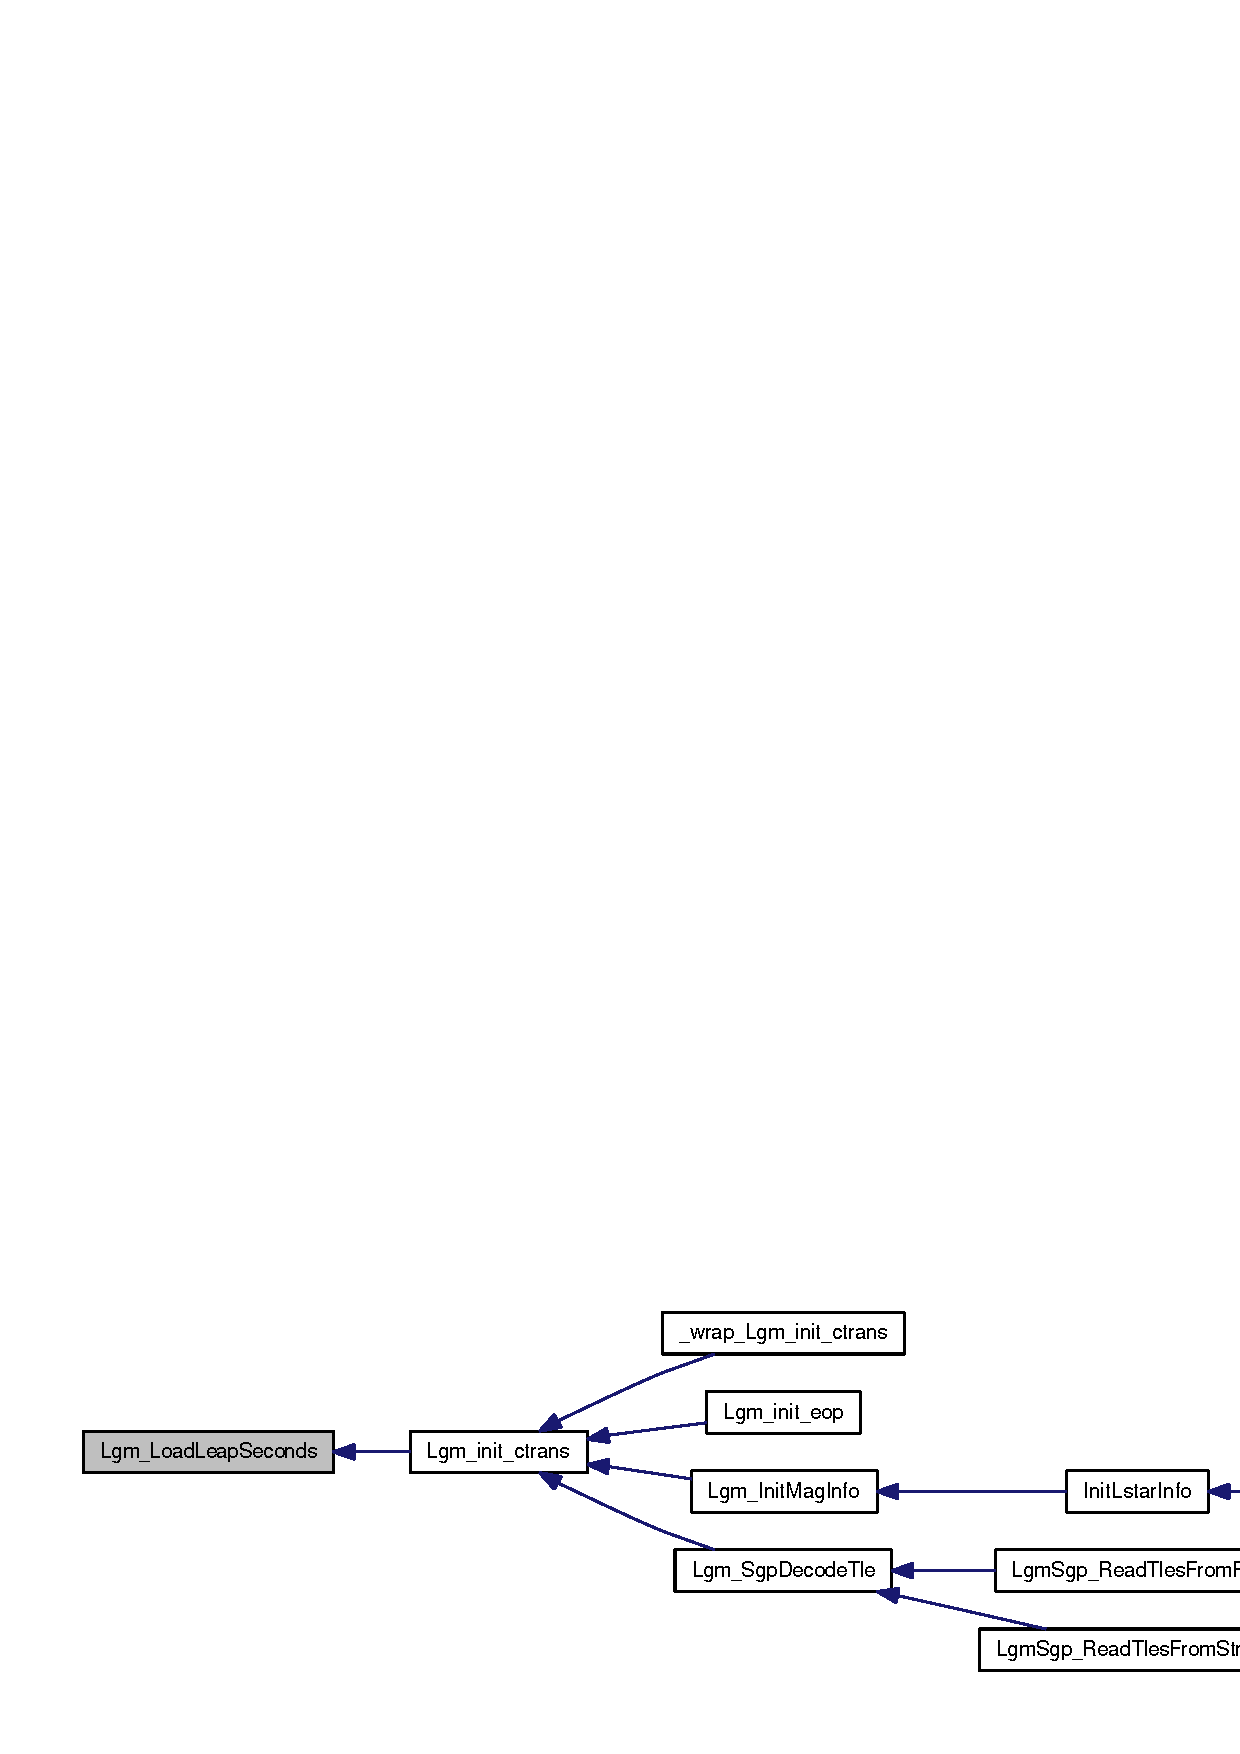
\includegraphics[width=391pt]{_lgm___date_and_time_8c_ffe919b2830c07067e255ca1a454a05a_icgraph}
\end{center}
\end{figure}
\hypertarget{_lgm___date_and_time_8c_38a6c5c43a1767d6f26c90f7970882e0}{
\index{Lgm\_\-DateAndTime.c@{Lgm\_\-DateAndTime.c}!Lgm\_\-TAI\_\-to\_\-GPS@{Lgm\_\-TAI\_\-to\_\-GPS}}
\index{Lgm\_\-TAI\_\-to\_\-GPS@{Lgm\_\-TAI\_\-to\_\-GPS}!Lgm_DateAndTime.c@{Lgm\_\-DateAndTime.c}}
\subsubsection[{Lgm\_\-TAI\_\-to\_\-GPS}]{\setlength{\rightskip}{0pt plus 5cm}void Lgm\_\-TAI\_\-to\_\-GPS ({\bf Lgm\_\-DateTime} $\ast$ {\em TAI}, \/  {\bf Lgm\_\-DateTime} $\ast$ {\em GPS}, \/  {\bf Lgm\_\-CTrans} $\ast$ {\em c})}}
\label{_lgm___date_and_time_8c_38a6c5c43a1767d6f26c90f7970882e0}




Definition at line 267 of file Lgm\_\-DateAndTime.c.

Here is the call graph for this function:\nopagebreak
\begin{figure}[H]
\begin{center}
\leavevmode
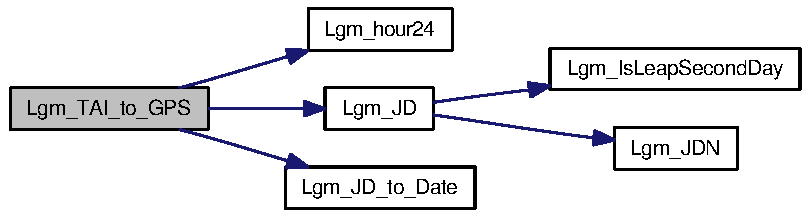
\includegraphics[width=212pt]{_lgm___date_and_time_8c_38a6c5c43a1767d6f26c90f7970882e0_cgraph}
\end{center}
\end{figure}


Here is the caller graph for this function:\nopagebreak
\begin{figure}[H]
\begin{center}
\leavevmode
\includegraphics[width=223pt]{_lgm___date_and_time_8c_38a6c5c43a1767d6f26c90f7970882e0_icgraph}
\end{center}
\end{figure}
\hypertarget{_lgm___date_and_time_8c_ae7db2b4a40466c781a6a29f91a51133}{
\index{Lgm\_\-DateAndTime.c@{Lgm\_\-DateAndTime.c}!Lgm\_\-GPS\_\-to\_\-TAI@{Lgm\_\-GPS\_\-to\_\-TAI}}
\index{Lgm\_\-GPS\_\-to\_\-TAI@{Lgm\_\-GPS\_\-to\_\-TAI}!Lgm_DateAndTime.c@{Lgm\_\-DateAndTime.c}}
\subsubsection[{Lgm\_\-GPS\_\-to\_\-TAI}]{\setlength{\rightskip}{0pt plus 5cm}void Lgm\_\-GPS\_\-to\_\-TAI ({\bf Lgm\_\-DateTime} $\ast$ {\em GPS}, \/  {\bf Lgm\_\-DateTime} $\ast$ {\em TAI}, \/  {\bf Lgm\_\-CTrans} $\ast$ {\em c})}}
\label{_lgm___date_and_time_8c_ae7db2b4a40466c781a6a29f91a51133}




Definition at line 282 of file Lgm\_\-DateAndTime.c.

Here is the call graph for this function:\nopagebreak
\begin{figure}[H]
\begin{center}
\leavevmode
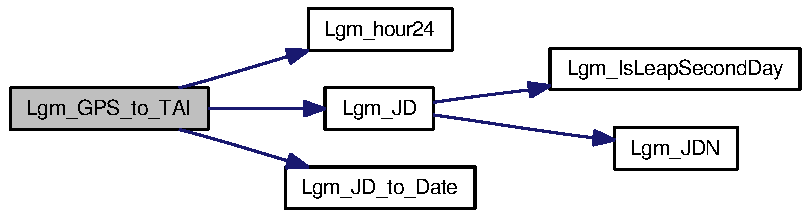
\includegraphics[width=212pt]{_lgm___date_and_time_8c_ae7db2b4a40466c781a6a29f91a51133_cgraph}
\end{center}
\end{figure}


Here is the caller graph for this function:\nopagebreak
\begin{figure}[H]
\begin{center}
\leavevmode
\includegraphics[width=223pt]{_lgm___date_and_time_8c_ae7db2b4a40466c781a6a29f91a51133_icgraph}
\end{center}
\end{figure}
\hypertarget{_lgm___date_and_time_8c_ab03f400cbc08ffa12348eb15bf37eb5}{
\index{Lgm\_\-DateAndTime.c@{Lgm\_\-DateAndTime.c}!Lgm\_\-UTC\_\-to\_\-GPS@{Lgm\_\-UTC\_\-to\_\-GPS}}
\index{Lgm\_\-UTC\_\-to\_\-GPS@{Lgm\_\-UTC\_\-to\_\-GPS}!Lgm_DateAndTime.c@{Lgm\_\-DateAndTime.c}}
\subsubsection[{Lgm\_\-UTC\_\-to\_\-GPS}]{\setlength{\rightskip}{0pt plus 5cm}void Lgm\_\-UTC\_\-to\_\-GPS ({\bf Lgm\_\-DateTime} $\ast$ {\em UTC}, \/  {\bf Lgm\_\-DateTime} $\ast$ {\em GPS}, \/  {\bf Lgm\_\-CTrans} $\ast$ {\em c})}}
\label{_lgm___date_and_time_8c_ab03f400cbc08ffa12348eb15bf37eb5}




Definition at line 303 of file Lgm\_\-DateAndTime.c.

Here is the call graph for this function:\nopagebreak
\begin{figure}[H]
\begin{center}
\leavevmode
\includegraphics[width=292pt]{_lgm___date_and_time_8c_ab03f400cbc08ffa12348eb15bf37eb5_cgraph}
\end{center}
\end{figure}


Here is the caller graph for this function:\nopagebreak
\begin{figure}[H]
\begin{center}
\leavevmode
\includegraphics[width=157pt]{_lgm___date_and_time_8c_ab03f400cbc08ffa12348eb15bf37eb5_icgraph}
\end{center}
\end{figure}
\hypertarget{_lgm___date_and_time_8c_1ff96bc78656dfc6ab411f6b4d8993f1}{
\index{Lgm\_\-DateAndTime.c@{Lgm\_\-DateAndTime.c}!Lgm\_\-GPS\_\-to\_\-UTC@{Lgm\_\-GPS\_\-to\_\-UTC}}
\index{Lgm\_\-GPS\_\-to\_\-UTC@{Lgm\_\-GPS\_\-to\_\-UTC}!Lgm_DateAndTime.c@{Lgm\_\-DateAndTime.c}}
\subsubsection[{Lgm\_\-GPS\_\-to\_\-UTC}]{\setlength{\rightskip}{0pt plus 5cm}void Lgm\_\-GPS\_\-to\_\-UTC ({\bf Lgm\_\-DateTime} $\ast$ {\em GPS}, \/  {\bf Lgm\_\-DateTime} $\ast$ {\em UTC}, \/  {\bf Lgm\_\-CTrans} $\ast$ {\em c})}}
\label{_lgm___date_and_time_8c_1ff96bc78656dfc6ab411f6b4d8993f1}




Definition at line 317 of file Lgm\_\-DateAndTime.c.

Here is the call graph for this function:\nopagebreak
\begin{figure}[H]
\begin{center}
\leavevmode
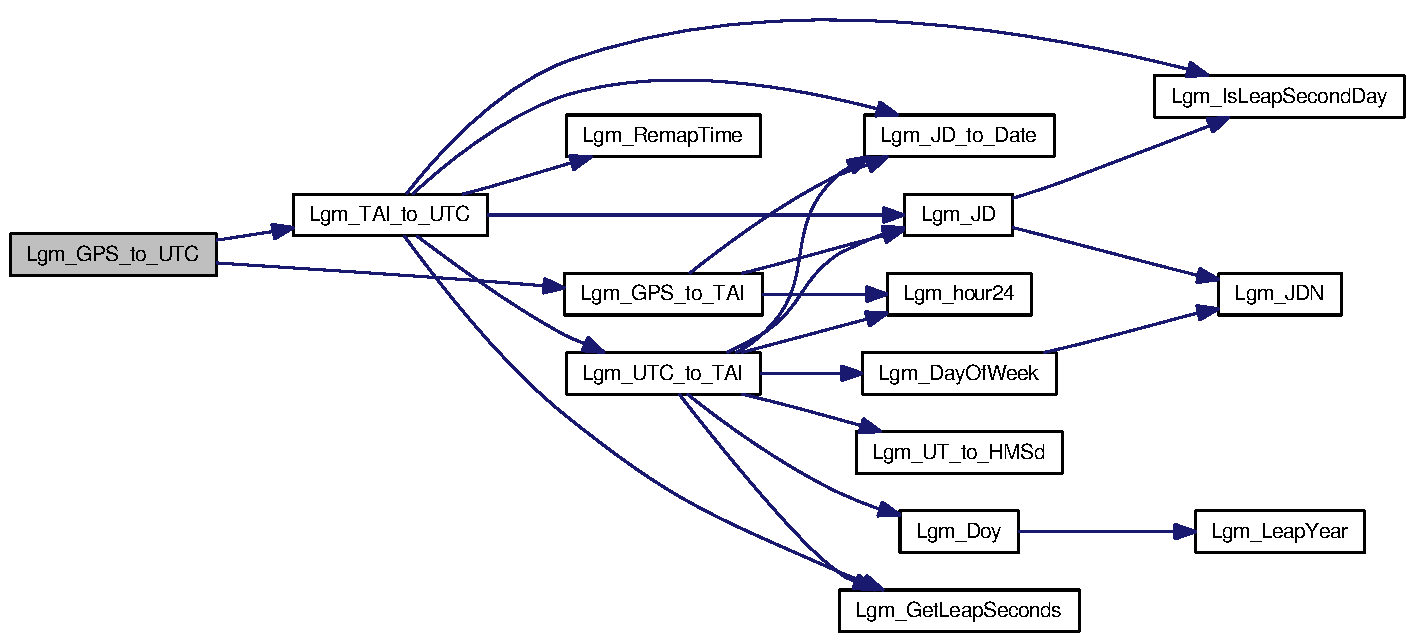
\includegraphics[width=357pt]{_lgm___date_and_time_8c_1ff96bc78656dfc6ab411f6b4d8993f1_cgraph}
\end{center}
\end{figure}


Here is the caller graph for this function:\nopagebreak
\begin{figure}[H]
\begin{center}
\leavevmode
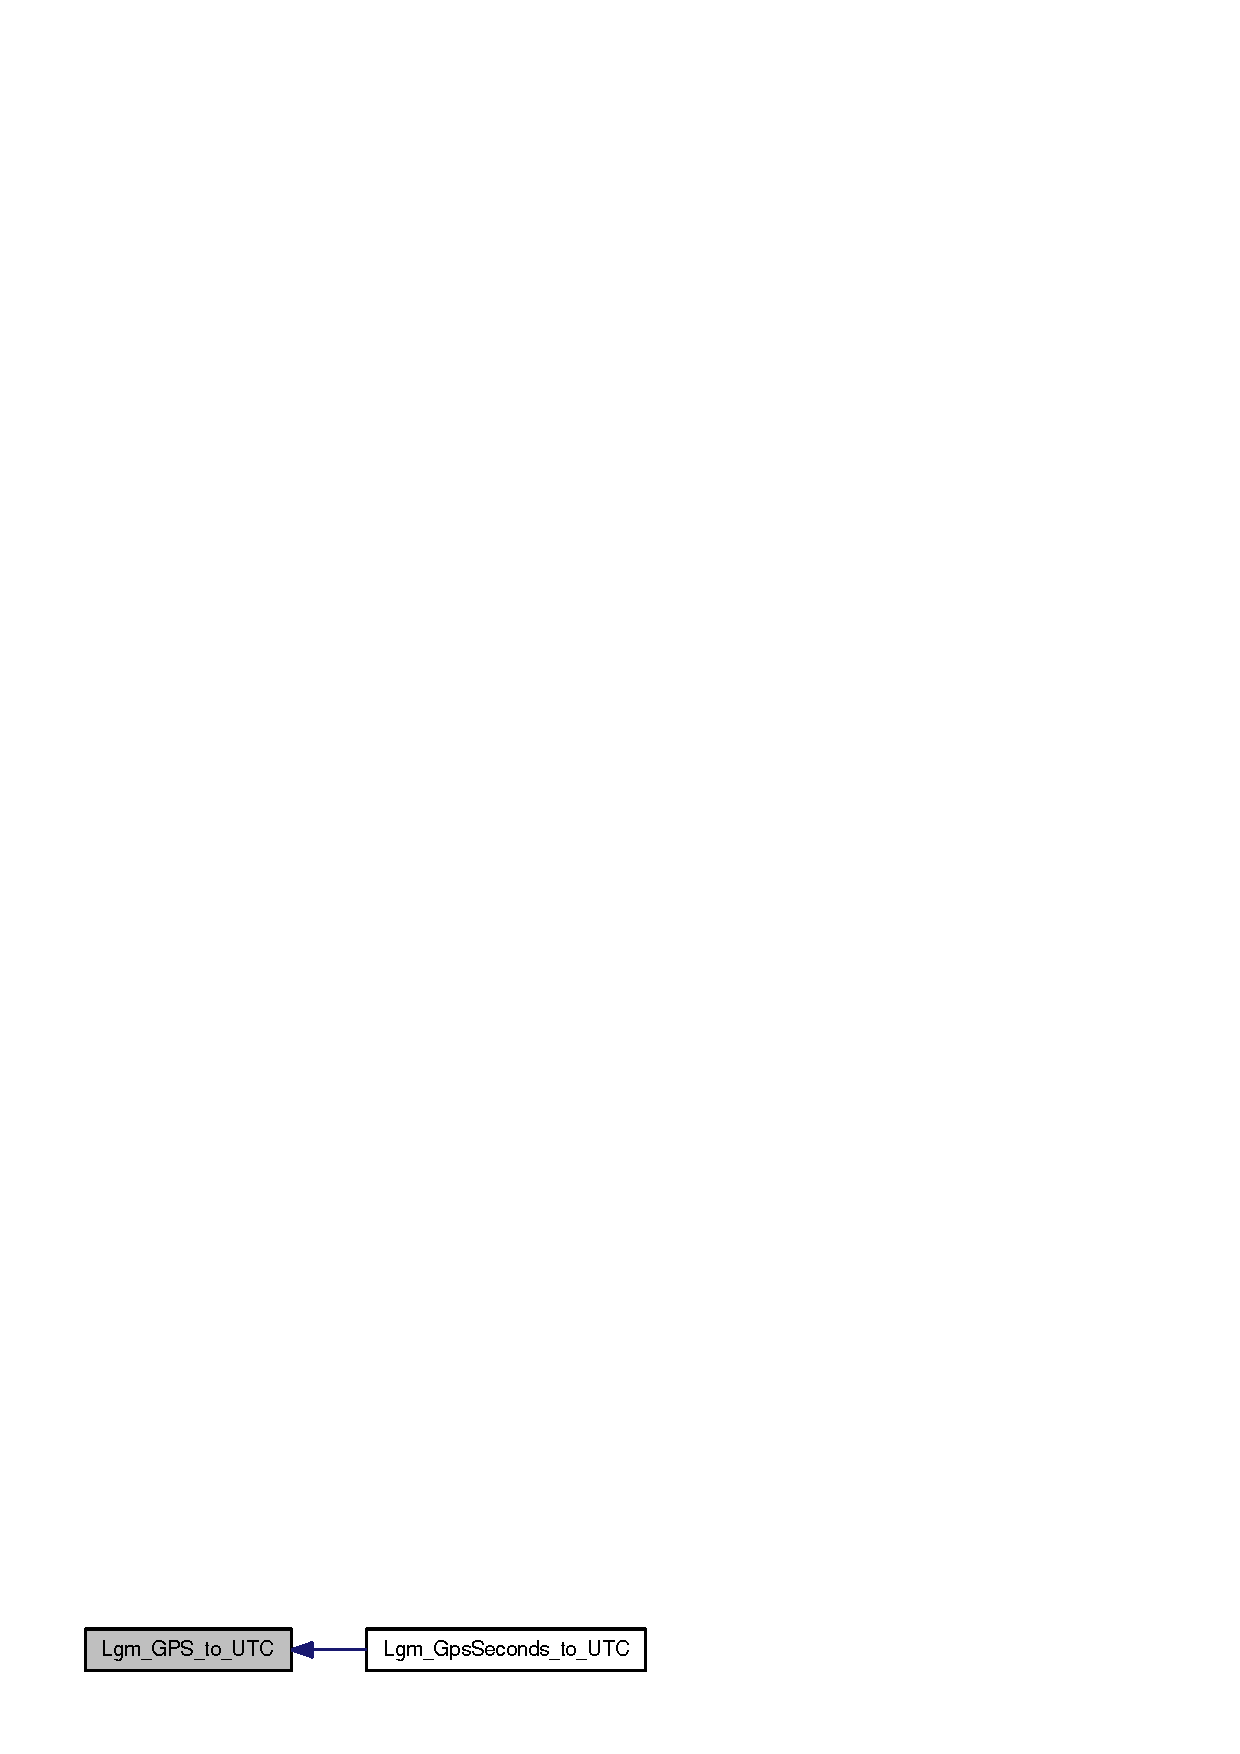
\includegraphics[width=157pt]{_lgm___date_and_time_8c_1ff96bc78656dfc6ab411f6b4d8993f1_icgraph}
\end{center}
\end{figure}
\hypertarget{_lgm___date_and_time_8c_62bc389169141b90c128c1413f10ba9a}{
\index{Lgm\_\-DateAndTime.c@{Lgm\_\-DateAndTime.c}!Lgm\_\-GPS\_\-to\_\-GpsSeconds@{Lgm\_\-GPS\_\-to\_\-GpsSeconds}}
\index{Lgm\_\-GPS\_\-to\_\-GpsSeconds@{Lgm\_\-GPS\_\-to\_\-GpsSeconds}!Lgm_DateAndTime.c@{Lgm\_\-DateAndTime.c}}
\subsubsection[{Lgm\_\-GPS\_\-to\_\-GpsSeconds}]{\setlength{\rightskip}{0pt plus 5cm}double Lgm\_\-GPS\_\-to\_\-GpsSeconds ({\bf Lgm\_\-DateTime} $\ast$ {\em GPS})}}
\label{_lgm___date_and_time_8c_62bc389169141b90c128c1413f10ba9a}




Definition at line 344 of file Lgm\_\-DateAndTime.c.

Here is the call graph for this function:\nopagebreak
\begin{figure}[H]
\begin{center}
\leavevmode
\includegraphics[width=138pt]{_lgm___date_and_time_8c_62bc389169141b90c128c1413f10ba9a_cgraph}
\end{center}
\end{figure}


Here is the caller graph for this function:\nopagebreak
\begin{figure}[H]
\begin{center}
\leavevmode
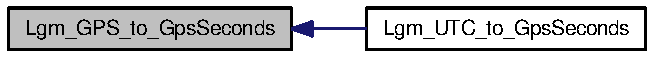
\includegraphics[width=175pt]{_lgm___date_and_time_8c_62bc389169141b90c128c1413f10ba9a_icgraph}
\end{center}
\end{figure}
\hypertarget{_lgm___date_and_time_8c_2170efd02fc5e37005be974bf1688753}{
\index{Lgm\_\-DateAndTime.c@{Lgm\_\-DateAndTime.c}!Lgm\_\-GpsSeconds\_\-to\_\-GPS@{Lgm\_\-GpsSeconds\_\-to\_\-GPS}}
\index{Lgm\_\-GpsSeconds\_\-to\_\-GPS@{Lgm\_\-GpsSeconds\_\-to\_\-GPS}!Lgm_DateAndTime.c@{Lgm\_\-DateAndTime.c}}
\subsubsection[{Lgm\_\-GpsSeconds\_\-to\_\-GPS}]{\setlength{\rightskip}{0pt plus 5cm}void Lgm\_\-GpsSeconds\_\-to\_\-GPS (double {\em GpsSeconds}, \/  {\bf Lgm\_\-DateTime} $\ast$ {\em GPS})}}
\label{_lgm___date_and_time_8c_2170efd02fc5e37005be974bf1688753}




Definition at line 351 of file Lgm\_\-DateAndTime.c.

Here is the call graph for this function:\nopagebreak
\begin{figure}[H]
\begin{center}
\leavevmode
\includegraphics[width=153pt]{_lgm___date_and_time_8c_2170efd02fc5e37005be974bf1688753_cgraph}
\end{center}
\end{figure}


Here is the caller graph for this function:\nopagebreak
\begin{figure}[H]
\begin{center}
\leavevmode
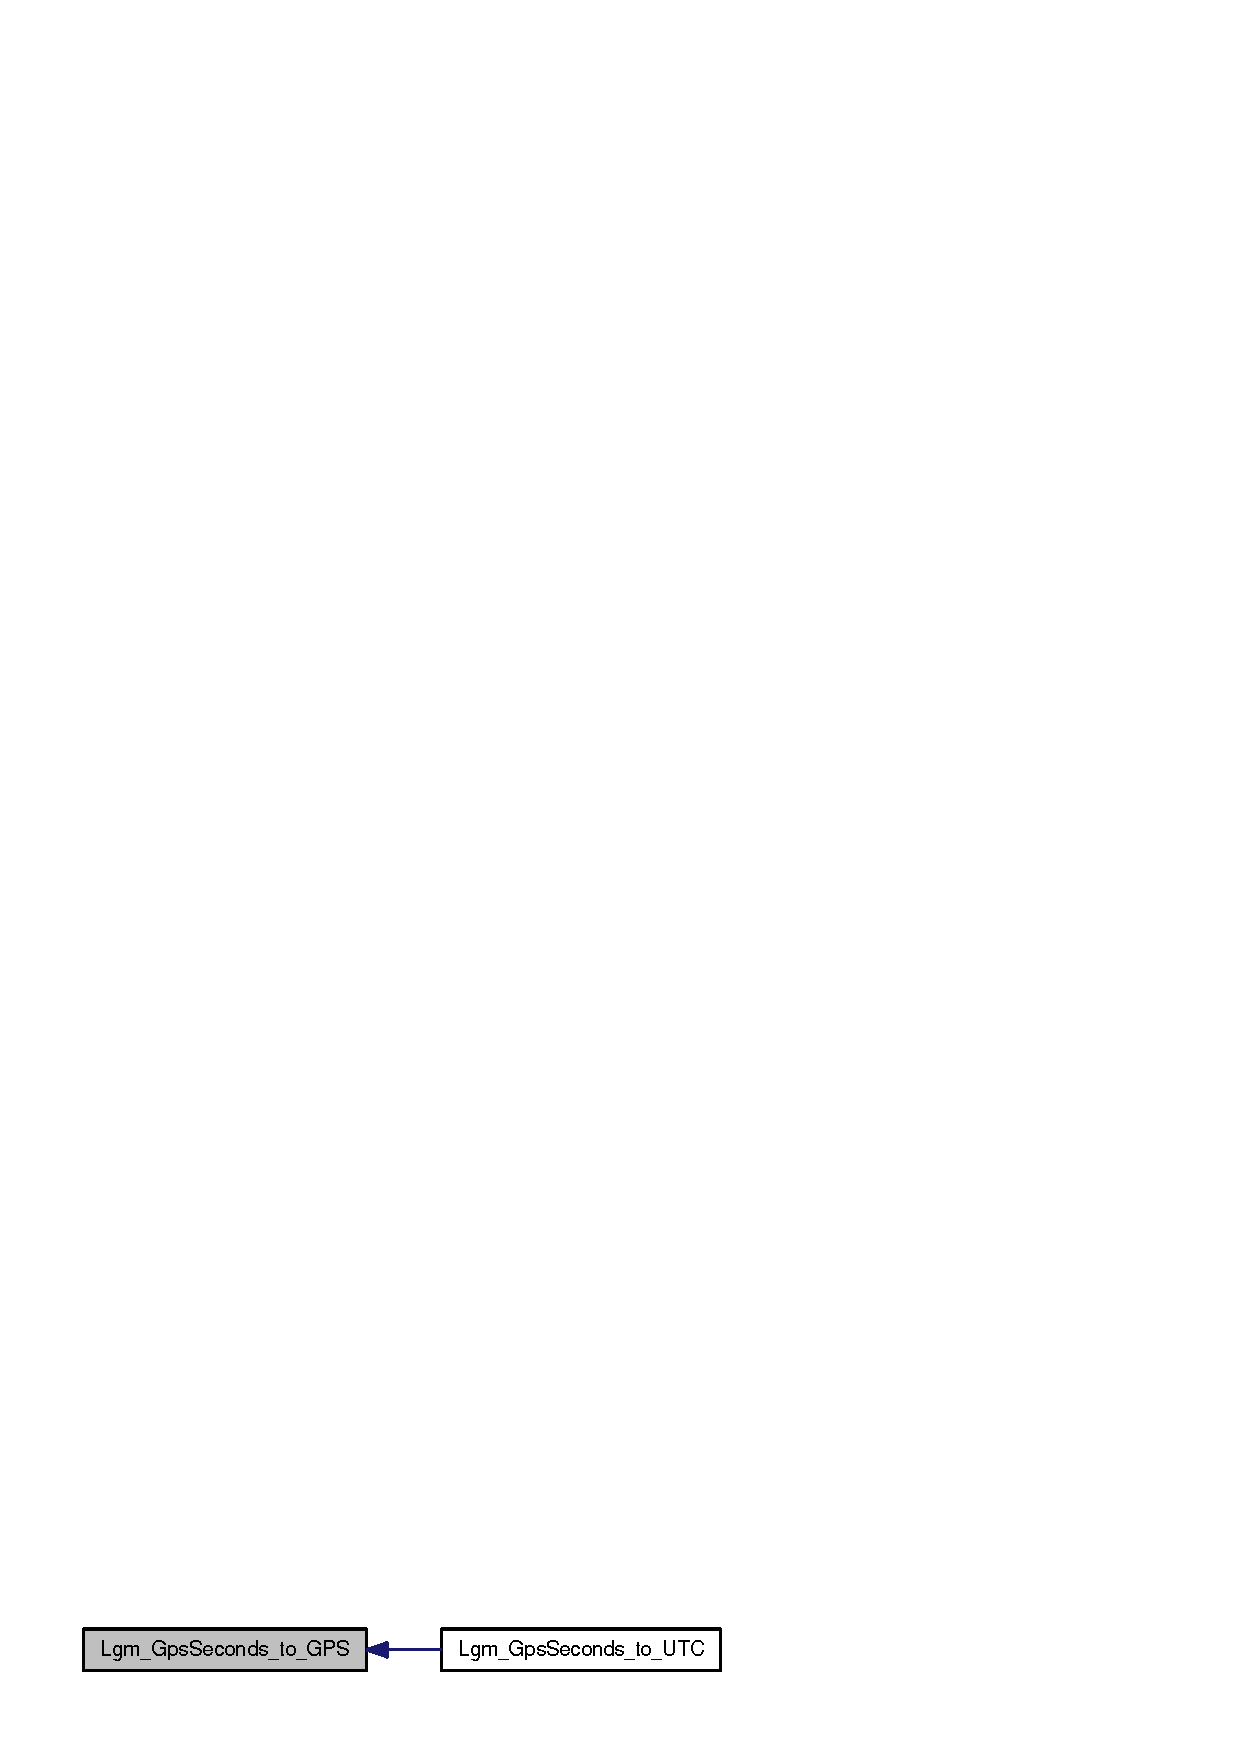
\includegraphics[width=175pt]{_lgm___date_and_time_8c_2170efd02fc5e37005be974bf1688753_icgraph}
\end{center}
\end{figure}
\hypertarget{_lgm___date_and_time_8c_e359f512f21bf55270e5454b9089cf2f}{
\index{Lgm\_\-DateAndTime.c@{Lgm\_\-DateAndTime.c}!Lgm\_\-GpsSeconds\_\-to\_\-UTC@{Lgm\_\-GpsSeconds\_\-to\_\-UTC}}
\index{Lgm\_\-GpsSeconds\_\-to\_\-UTC@{Lgm\_\-GpsSeconds\_\-to\_\-UTC}!Lgm_DateAndTime.c@{Lgm\_\-DateAndTime.c}}
\subsubsection[{Lgm\_\-GpsSeconds\_\-to\_\-UTC}]{\setlength{\rightskip}{0pt plus 5cm}void Lgm\_\-GpsSeconds\_\-to\_\-UTC (double {\em GpsSeconds}, \/  {\bf Lgm\_\-DateTime} $\ast$ {\em UTC}, \/  {\bf Lgm\_\-CTrans} $\ast$ {\em c})}}
\label{_lgm___date_and_time_8c_e359f512f21bf55270e5454b9089cf2f}




Definition at line 366 of file Lgm\_\-DateAndTime.c.

Here is the call graph for this function:\nopagebreak
\begin{figure}[H]
\begin{center}
\leavevmode
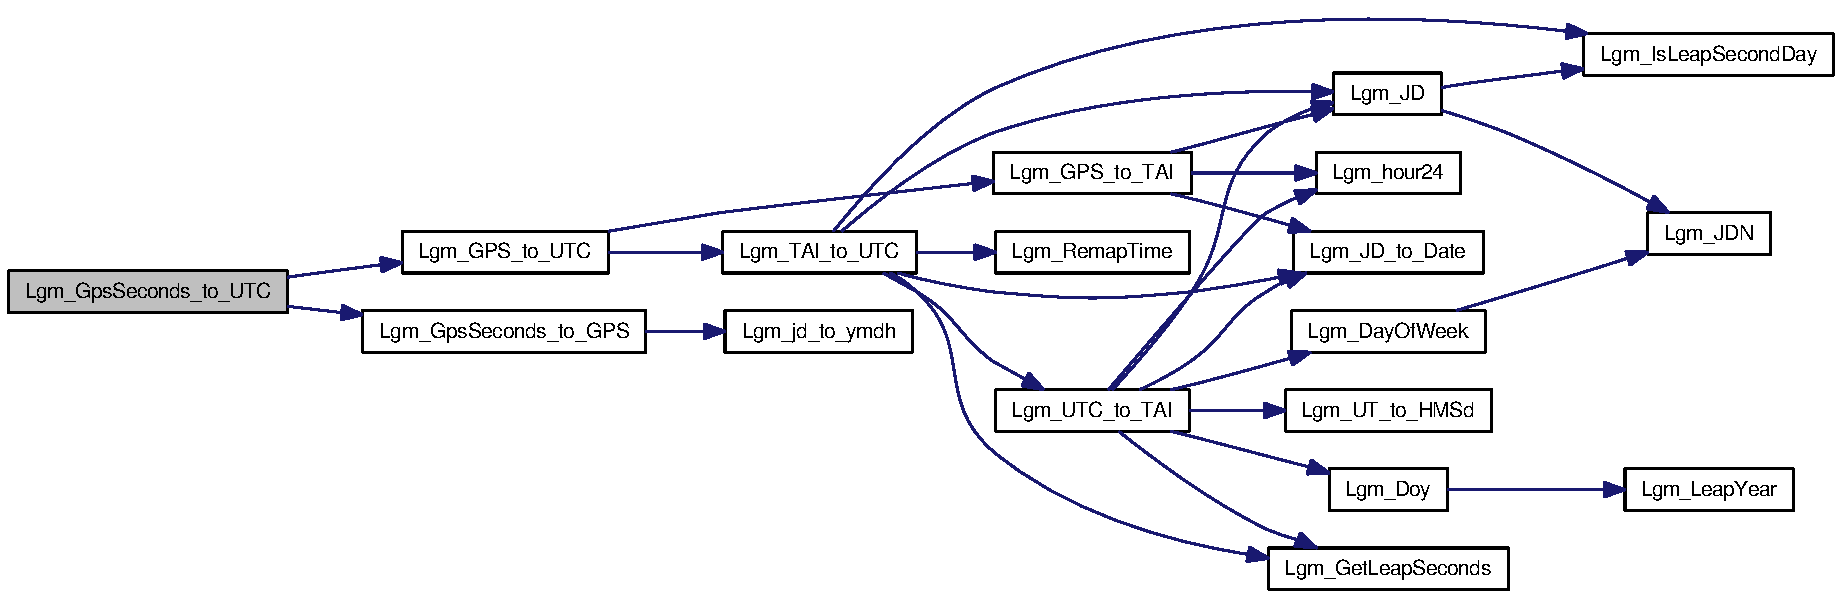
\includegraphics[width=420pt]{_lgm___date_and_time_8c_e359f512f21bf55270e5454b9089cf2f_cgraph}
\end{center}
\end{figure}
\hypertarget{_lgm___date_and_time_8c_a242e28151e439aefeb83cd85c735903}{
\index{Lgm\_\-DateAndTime.c@{Lgm\_\-DateAndTime.c}!Lgm\_\-UTC\_\-to\_\-GpsSeconds@{Lgm\_\-UTC\_\-to\_\-GpsSeconds}}
\index{Lgm\_\-UTC\_\-to\_\-GpsSeconds@{Lgm\_\-UTC\_\-to\_\-GpsSeconds}!Lgm_DateAndTime.c@{Lgm\_\-DateAndTime.c}}
\subsubsection[{Lgm\_\-UTC\_\-to\_\-GpsSeconds}]{\setlength{\rightskip}{0pt plus 5cm}double Lgm\_\-UTC\_\-to\_\-GpsSeconds ({\bf Lgm\_\-DateTime} $\ast$ {\em UTC}, \/  {\bf Lgm\_\-CTrans} $\ast$ {\em c})}}
\label{_lgm___date_and_time_8c_a242e28151e439aefeb83cd85c735903}




Definition at line 373 of file Lgm\_\-DateAndTime.c.

Here is the call graph for this function:\nopagebreak
\begin{figure}[H]
\begin{center}
\leavevmode
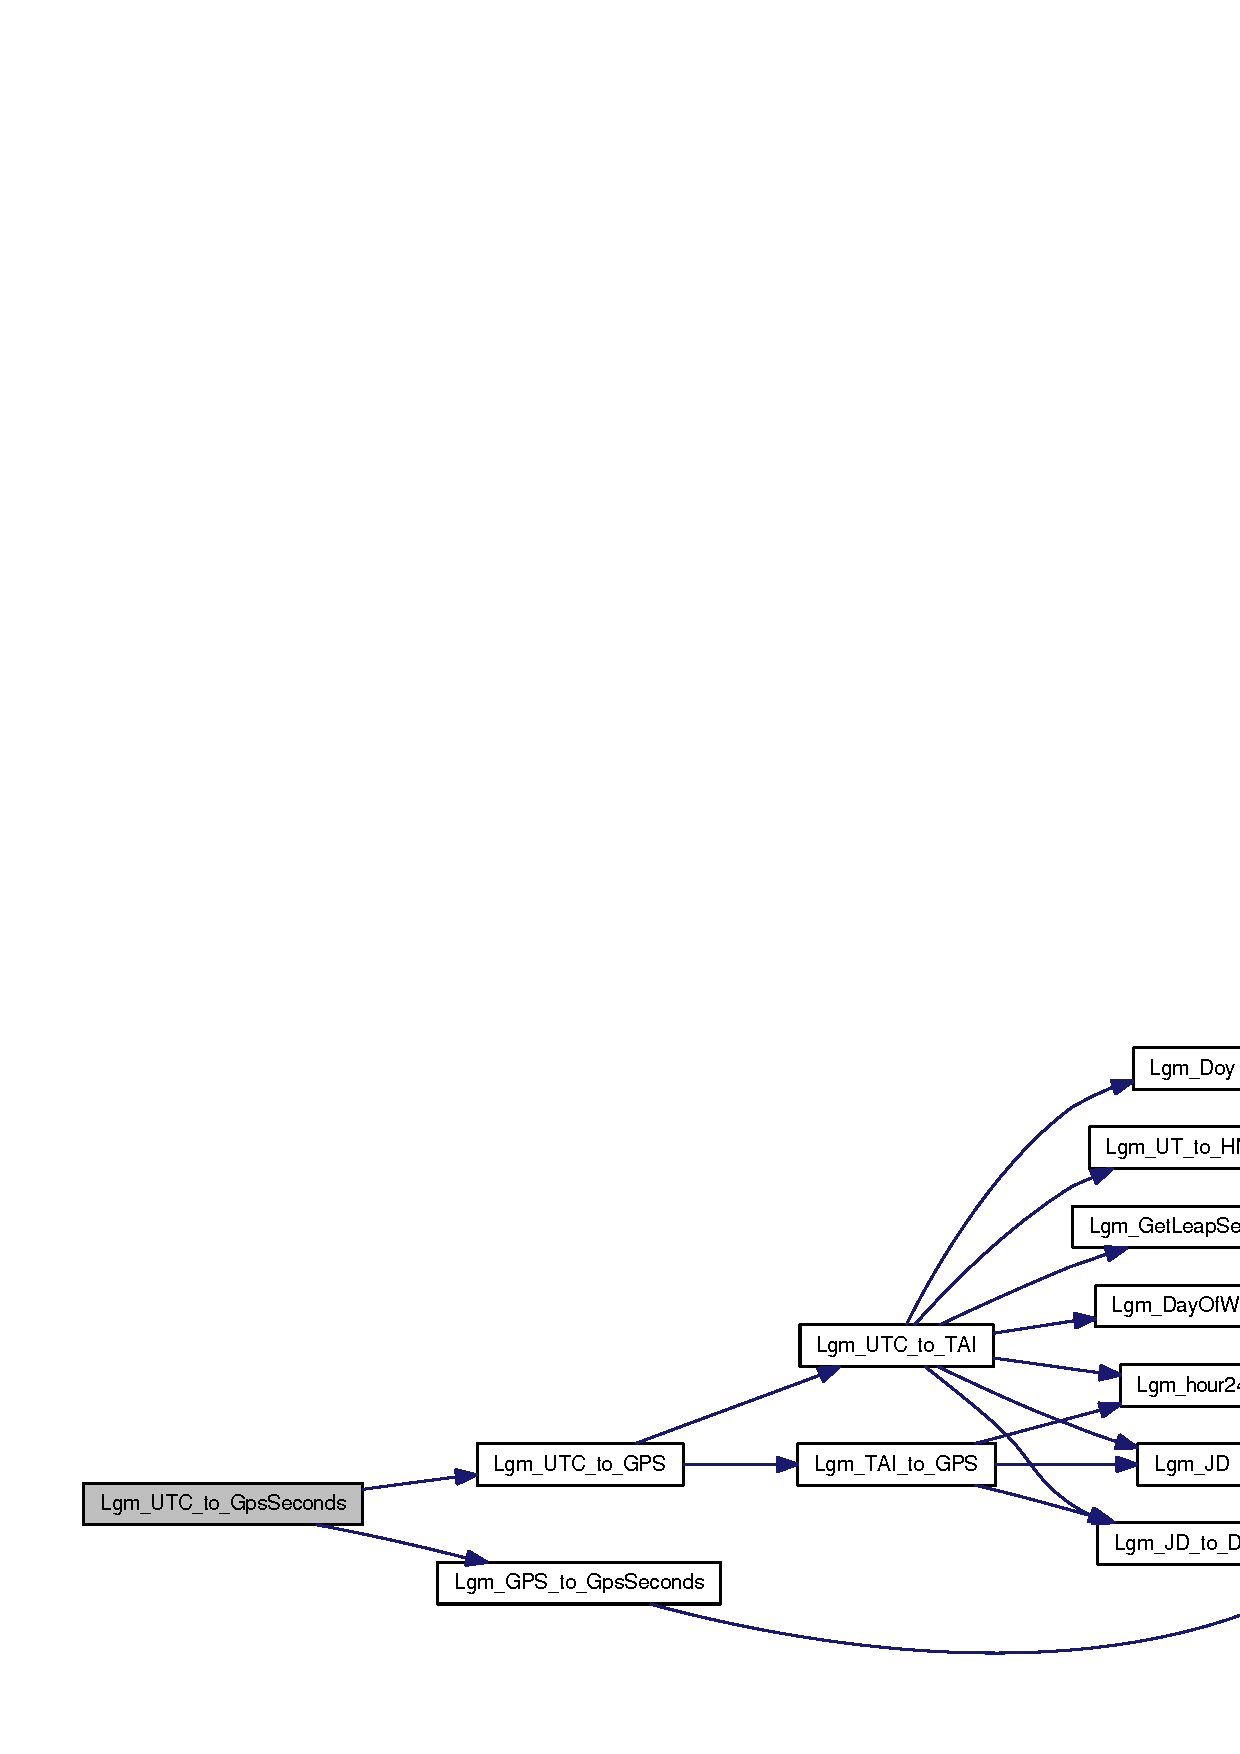
\includegraphics[width=395pt]{_lgm___date_and_time_8c_a242e28151e439aefeb83cd85c735903_cgraph}
\end{center}
\end{figure}
\hypertarget{_lgm___date_and_time_8c_8d1a12a1442f0fed2e64749c47db8157}{
\index{Lgm\_\-DateAndTime.c@{Lgm\_\-DateAndTime.c}!Lgm\_\-TAI\_\-to\_\-TaiSeconds@{Lgm\_\-TAI\_\-to\_\-TaiSeconds}}
\index{Lgm\_\-TAI\_\-to\_\-TaiSeconds@{Lgm\_\-TAI\_\-to\_\-TaiSeconds}!Lgm_DateAndTime.c@{Lgm\_\-DateAndTime.c}}
\subsubsection[{Lgm\_\-TAI\_\-to\_\-TaiSeconds}]{\setlength{\rightskip}{0pt plus 5cm}double Lgm\_\-TAI\_\-to\_\-TaiSeconds ({\bf Lgm\_\-DateTime} $\ast$ {\em TAI})}}
\label{_lgm___date_and_time_8c_8d1a12a1442f0fed2e64749c47db8157}




Definition at line 392 of file Lgm\_\-DateAndTime.c.

Here is the call graph for this function:\nopagebreak
\begin{figure}[H]
\begin{center}
\leavevmode
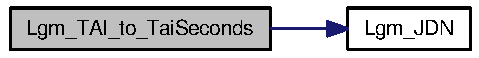
\includegraphics[width=133pt]{_lgm___date_and_time_8c_8d1a12a1442f0fed2e64749c47db8157_cgraph}
\end{center}
\end{figure}


Here is the caller graph for this function:\nopagebreak
\begin{figure}[H]
\begin{center}
\leavevmode
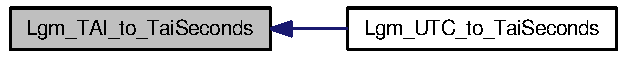
\includegraphics[width=168pt]{_lgm___date_and_time_8c_8d1a12a1442f0fed2e64749c47db8157_icgraph}
\end{center}
\end{figure}
\hypertarget{_lgm___date_and_time_8c_39c239611e99c1ad3a2ae8af2cb93d9c}{
\index{Lgm\_\-DateAndTime.c@{Lgm\_\-DateAndTime.c}!Lgm\_\-TaiSeconds\_\-to\_\-TAI@{Lgm\_\-TaiSeconds\_\-to\_\-TAI}}
\index{Lgm\_\-TaiSeconds\_\-to\_\-TAI@{Lgm\_\-TaiSeconds\_\-to\_\-TAI}!Lgm_DateAndTime.c@{Lgm\_\-DateAndTime.c}}
\subsubsection[{Lgm\_\-TaiSeconds\_\-to\_\-TAI}]{\setlength{\rightskip}{0pt plus 5cm}void Lgm\_\-TaiSeconds\_\-to\_\-TAI (double {\em TaiSeconds}, \/  {\bf Lgm\_\-DateTime} $\ast$ {\em TAI})}}
\label{_lgm___date_and_time_8c_39c239611e99c1ad3a2ae8af2cb93d9c}




Definition at line 399 of file Lgm\_\-DateAndTime.c.

Here is the call graph for this function:\nopagebreak
\begin{figure}[H]
\begin{center}
\leavevmode
\includegraphics[width=148pt]{_lgm___date_and_time_8c_39c239611e99c1ad3a2ae8af2cb93d9c_cgraph}
\end{center}
\end{figure}


Here is the caller graph for this function:\nopagebreak
\begin{figure}[H]
\begin{center}
\leavevmode
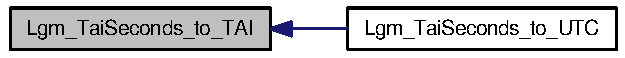
\includegraphics[width=168pt]{_lgm___date_and_time_8c_39c239611e99c1ad3a2ae8af2cb93d9c_icgraph}
\end{center}
\end{figure}
\hypertarget{_lgm___date_and_time_8c_906b9059ecb4e21fa8bf26b91df3dbad}{
\index{Lgm\_\-DateAndTime.c@{Lgm\_\-DateAndTime.c}!Lgm\_\-TaiSeconds\_\-to\_\-UTC@{Lgm\_\-TaiSeconds\_\-to\_\-UTC}}
\index{Lgm\_\-TaiSeconds\_\-to\_\-UTC@{Lgm\_\-TaiSeconds\_\-to\_\-UTC}!Lgm_DateAndTime.c@{Lgm\_\-DateAndTime.c}}
\subsubsection[{Lgm\_\-TaiSeconds\_\-to\_\-UTC}]{\setlength{\rightskip}{0pt plus 5cm}void Lgm\_\-TaiSeconds\_\-to\_\-UTC (double {\em TaiSeconds}, \/  {\bf Lgm\_\-DateTime} $\ast$ {\em UTC}, \/  {\bf Lgm\_\-CTrans} $\ast$ {\em c})}}
\label{_lgm___date_and_time_8c_906b9059ecb4e21fa8bf26b91df3dbad}




Definition at line 414 of file Lgm\_\-DateAndTime.c.

Here is the call graph for this function:\nopagebreak
\begin{figure}[H]
\begin{center}
\leavevmode
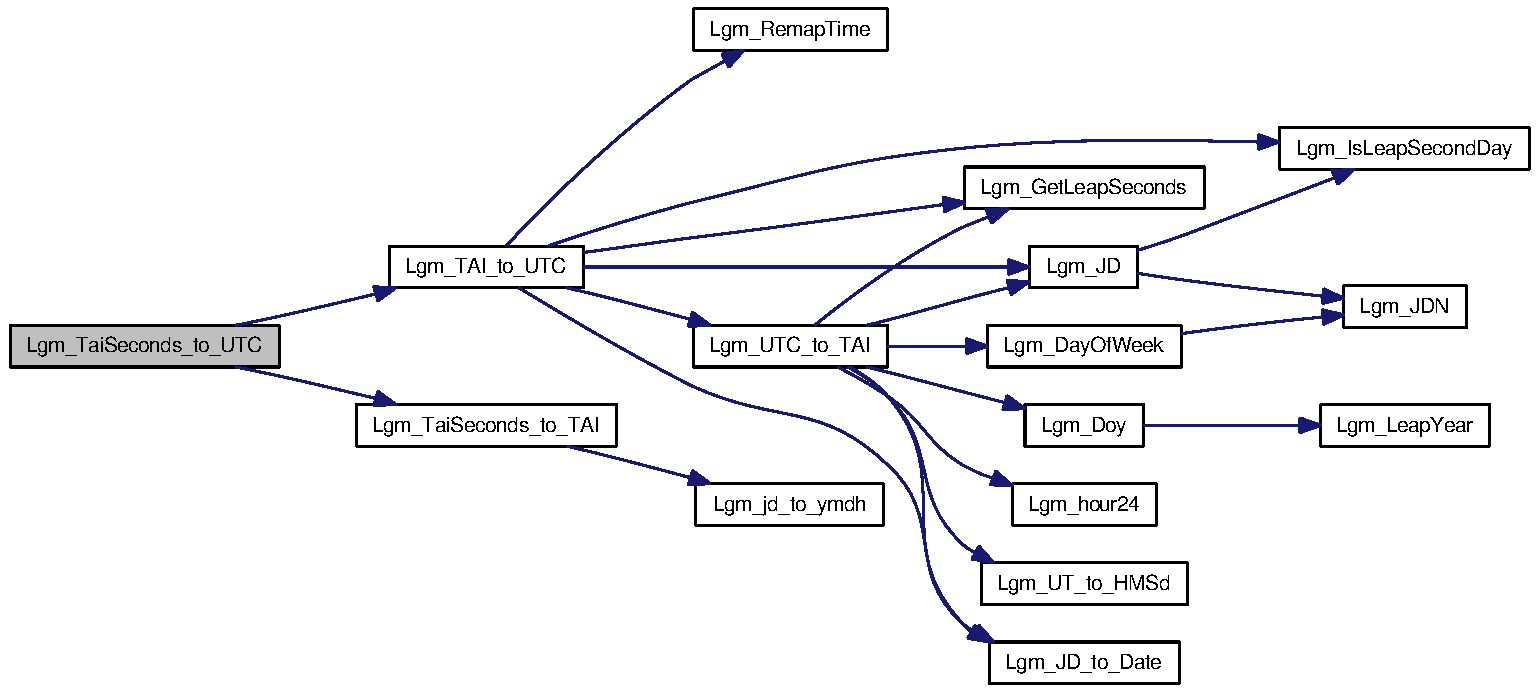
\includegraphics[width=387pt]{_lgm___date_and_time_8c_906b9059ecb4e21fa8bf26b91df3dbad_cgraph}
\end{center}
\end{figure}
\hypertarget{_lgm___date_and_time_8c_9c99186b444f75dd856bd789298b9cb8}{
\index{Lgm\_\-DateAndTime.c@{Lgm\_\-DateAndTime.c}!Lgm\_\-UTC\_\-to\_\-TaiSeconds@{Lgm\_\-UTC\_\-to\_\-TaiSeconds}}
\index{Lgm\_\-UTC\_\-to\_\-TaiSeconds@{Lgm\_\-UTC\_\-to\_\-TaiSeconds}!Lgm_DateAndTime.c@{Lgm\_\-DateAndTime.c}}
\subsubsection[{Lgm\_\-UTC\_\-to\_\-TaiSeconds}]{\setlength{\rightskip}{0pt plus 5cm}double Lgm\_\-UTC\_\-to\_\-TaiSeconds ({\bf Lgm\_\-DateTime} $\ast$ {\em UTC}, \/  {\bf Lgm\_\-CTrans} $\ast$ {\em c})}}
\label{_lgm___date_and_time_8c_9c99186b444f75dd856bd789298b9cb8}




Definition at line 421 of file Lgm\_\-DateAndTime.c.

Here is the call graph for this function:\nopagebreak
\begin{figure}[H]
\begin{center}
\leavevmode
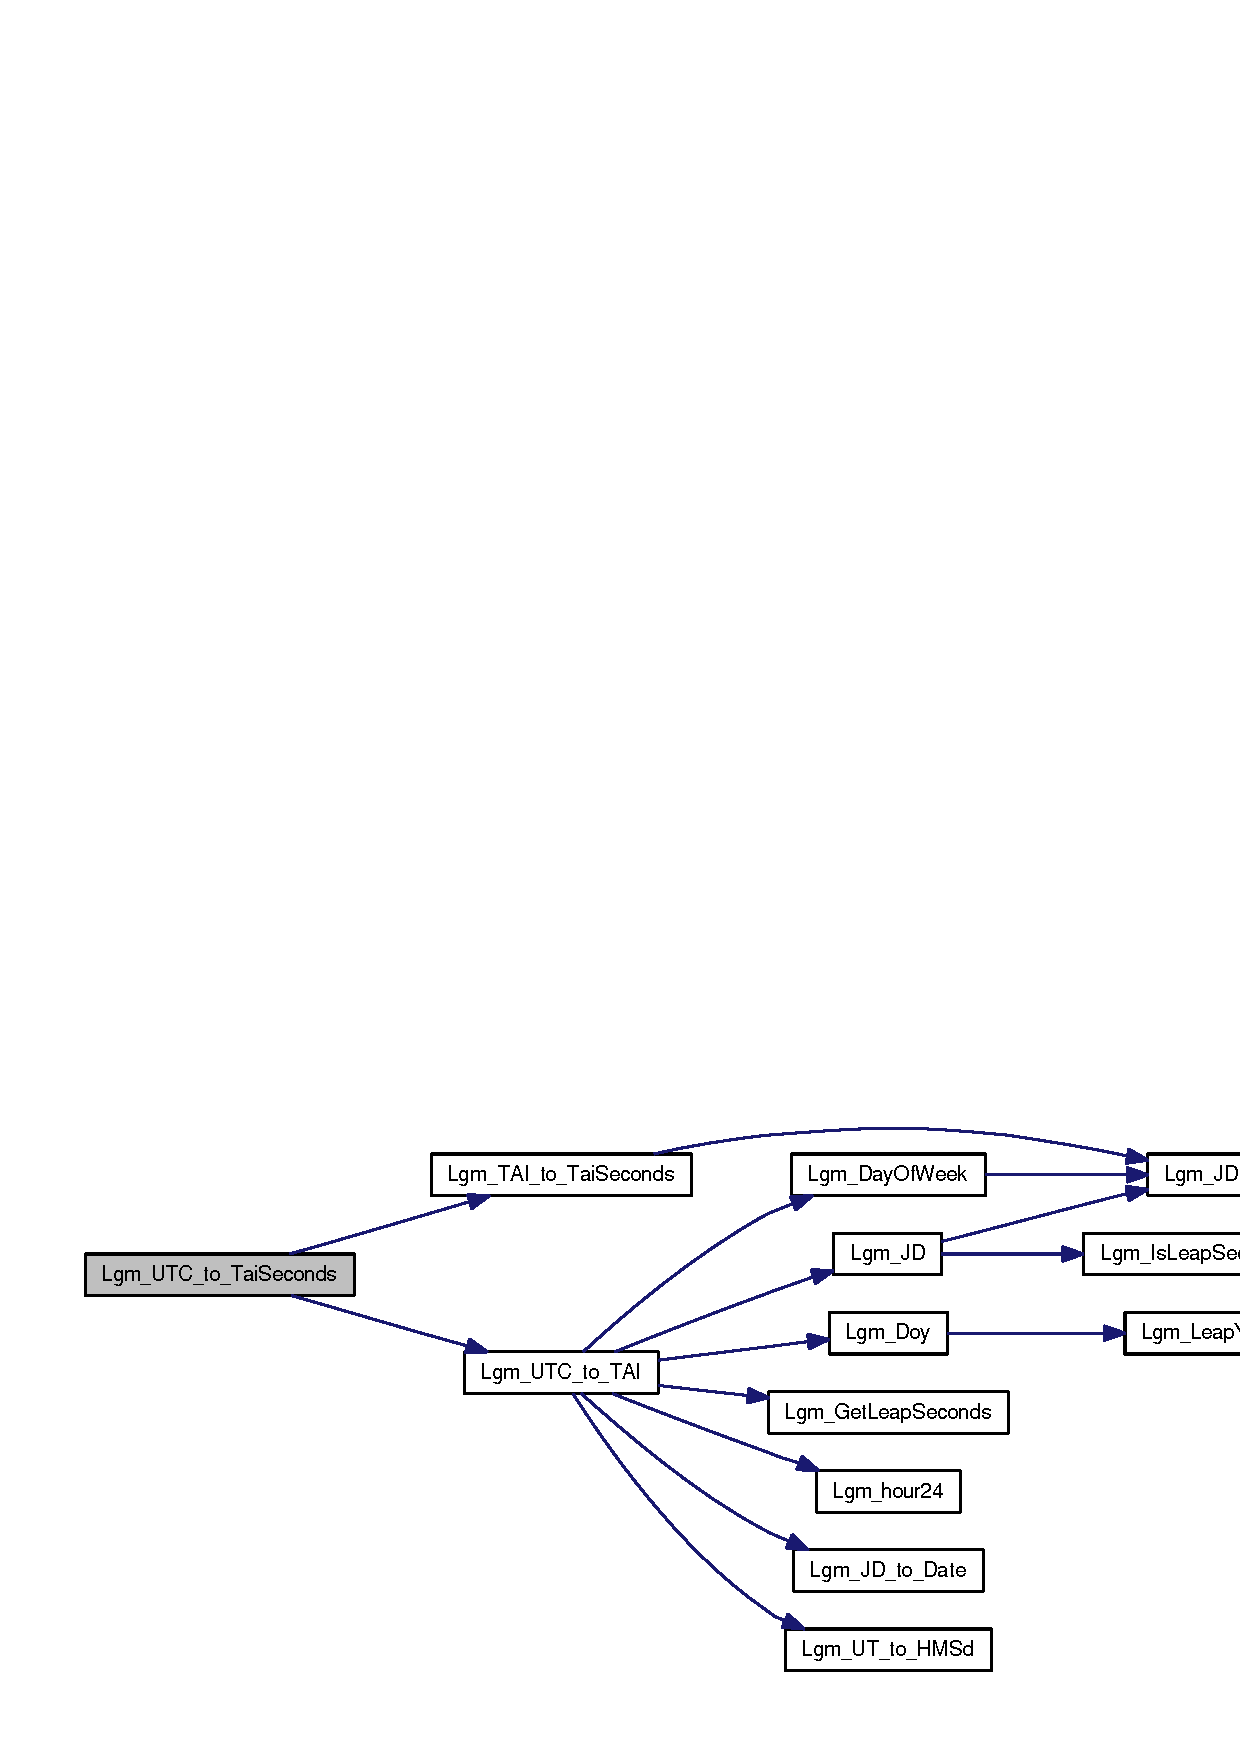
\includegraphics[width=322pt]{_lgm___date_and_time_8c_9c99186b444f75dd856bd789298b9cb8_cgraph}
\end{center}
\end{figure}
\hypertarget{_lgm___date_and_time_8c_fc2358593ed2c075d04b1ae6663a86a6}{
\index{Lgm\_\-DateAndTime.c@{Lgm\_\-DateAndTime.c}!Lgm\_\-UTC\_\-to\_\-TAI@{Lgm\_\-UTC\_\-to\_\-TAI}}
\index{Lgm\_\-UTC\_\-to\_\-TAI@{Lgm\_\-UTC\_\-to\_\-TAI}!Lgm_DateAndTime.c@{Lgm\_\-DateAndTime.c}}
\subsubsection[{Lgm\_\-UTC\_\-to\_\-TAI}]{\setlength{\rightskip}{0pt plus 5cm}void Lgm\_\-UTC\_\-to\_\-TAI ({\bf Lgm\_\-DateTime} $\ast$ {\em UTC}, \/  {\bf Lgm\_\-DateTime} $\ast$ {\em TAI}, \/  {\bf Lgm\_\-CTrans} $\ast$ {\em c})}}
\label{_lgm___date_and_time_8c_fc2358593ed2c075d04b1ae6663a86a6}




Definition at line 438 of file Lgm\_\-DateAndTime.c.

Here is the call graph for this function:\nopagebreak
\begin{figure}[H]
\begin{center}
\leavevmode
\includegraphics[width=223pt]{_lgm___date_and_time_8c_fc2358593ed2c075d04b1ae6663a86a6_cgraph}
\end{center}
\end{figure}


Here is the caller graph for this function:\nopagebreak
\begin{figure}[H]
\begin{center}
\leavevmode
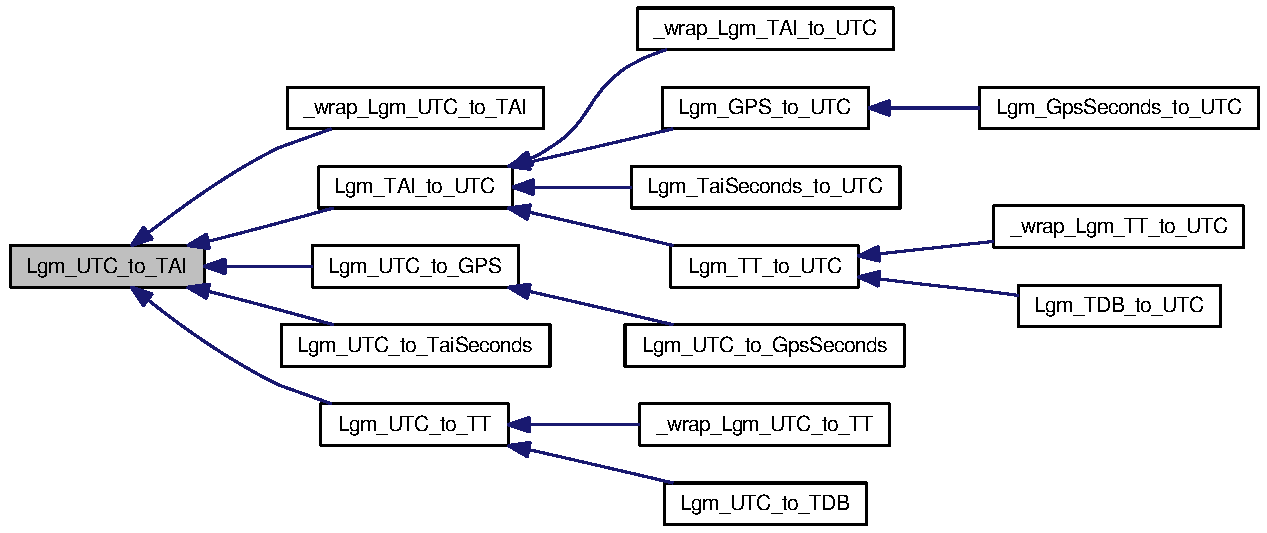
\includegraphics[width=322pt]{_lgm___date_and_time_8c_fc2358593ed2c075d04b1ae6663a86a6_icgraph}
\end{center}
\end{figure}
\hypertarget{_lgm___date_and_time_8c_de5bfe94202a0503dbbe1cb6a066ecf9}{
\index{Lgm\_\-DateAndTime.c@{Lgm\_\-DateAndTime.c}!Lgm\_\-TAI\_\-to\_\-UTC@{Lgm\_\-TAI\_\-to\_\-UTC}}
\index{Lgm\_\-TAI\_\-to\_\-UTC@{Lgm\_\-TAI\_\-to\_\-UTC}!Lgm_DateAndTime.c@{Lgm\_\-DateAndTime.c}}
\subsubsection[{Lgm\_\-TAI\_\-to\_\-UTC}]{\setlength{\rightskip}{0pt plus 5cm}void Lgm\_\-TAI\_\-to\_\-UTC ({\bf Lgm\_\-DateTime} $\ast$ {\em TAI}, \/  {\bf Lgm\_\-DateTime} $\ast$ {\em UTC}, \/  {\bf Lgm\_\-CTrans} $\ast$ {\em c})}}
\label{_lgm___date_and_time_8c_de5bfe94202a0503dbbe1cb6a066ecf9}




Definition at line 513 of file Lgm\_\-DateAndTime.c.

Here is the call graph for this function:\nopagebreak
\begin{figure}[H]
\begin{center}
\leavevmode
\includegraphics[width=288pt]{_lgm___date_and_time_8c_de5bfe94202a0503dbbe1cb6a066ecf9_cgraph}
\end{center}
\end{figure}


Here is the caller graph for this function:\nopagebreak
\begin{figure}[H]
\begin{center}
\leavevmode
\includegraphics[width=237pt]{_lgm___date_and_time_8c_de5bfe94202a0503dbbe1cb6a066ecf9_icgraph}
\end{center}
\end{figure}
\hypertarget{_lgm___date_and_time_8c_1c9dffe866b03fe6c519bba85445b8ef}{
\index{Lgm\_\-DateAndTime.c@{Lgm\_\-DateAndTime.c}!Lgm\_\-TT\_\-to\_\-TAI@{Lgm\_\-TT\_\-to\_\-TAI}}
\index{Lgm\_\-TT\_\-to\_\-TAI@{Lgm\_\-TT\_\-to\_\-TAI}!Lgm_DateAndTime.c@{Lgm\_\-DateAndTime.c}}
\subsubsection[{Lgm\_\-TT\_\-to\_\-TAI}]{\setlength{\rightskip}{0pt plus 5cm}void Lgm\_\-TT\_\-to\_\-TAI ({\bf Lgm\_\-DateTime} $\ast$ {\em TT}, \/  {\bf Lgm\_\-DateTime} $\ast$ {\em TAI}, \/  {\bf Lgm\_\-CTrans} $\ast$ {\em c})}}
\label{_lgm___date_and_time_8c_1c9dffe866b03fe6c519bba85445b8ef}




Definition at line 592 of file Lgm\_\-DateAndTime.c.

Here is the call graph for this function:\nopagebreak
\begin{figure}[H]
\begin{center}
\leavevmode
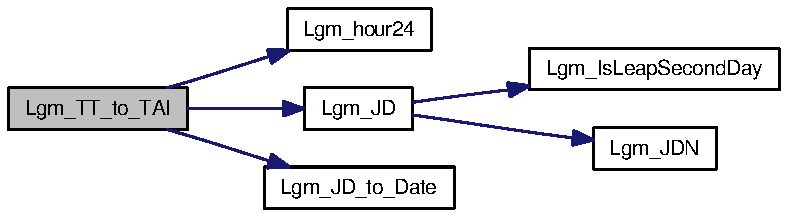
\includegraphics[width=207pt]{_lgm___date_and_time_8c_1c9dffe866b03fe6c519bba85445b8ef_cgraph}
\end{center}
\end{figure}


Here is the caller graph for this function:\nopagebreak
\begin{figure}[H]
\begin{center}
\leavevmode
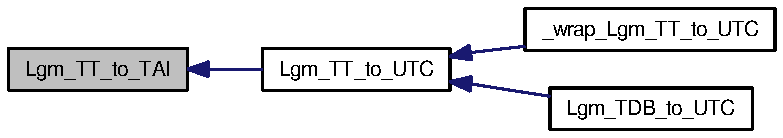
\includegraphics[width=206pt]{_lgm___date_and_time_8c_1c9dffe866b03fe6c519bba85445b8ef_icgraph}
\end{center}
\end{figure}
\hypertarget{_lgm___date_and_time_8c_df975a9192e9f08e25898ad3bdf906ff}{
\index{Lgm\_\-DateAndTime.c@{Lgm\_\-DateAndTime.c}!Lgm\_\-TAI\_\-to\_\-TT@{Lgm\_\-TAI\_\-to\_\-TT}}
\index{Lgm\_\-TAI\_\-to\_\-TT@{Lgm\_\-TAI\_\-to\_\-TT}!Lgm_DateAndTime.c@{Lgm\_\-DateAndTime.c}}
\subsubsection[{Lgm\_\-TAI\_\-to\_\-TT}]{\setlength{\rightskip}{0pt plus 5cm}void Lgm\_\-TAI\_\-to\_\-TT ({\bf Lgm\_\-DateTime} $\ast$ {\em TAI}, \/  {\bf Lgm\_\-DateTime} $\ast$ {\em TT}, \/  {\bf Lgm\_\-CTrans} $\ast$ {\em c})}}
\label{_lgm___date_and_time_8c_df975a9192e9f08e25898ad3bdf906ff}




Definition at line 614 of file Lgm\_\-DateAndTime.c.

Here is the call graph for this function:\nopagebreak
\begin{figure}[H]
\begin{center}
\leavevmode
\includegraphics[width=207pt]{_lgm___date_and_time_8c_df975a9192e9f08e25898ad3bdf906ff_cgraph}
\end{center}
\end{figure}
\hypertarget{_lgm___date_and_time_8c_22d70f08569629bfb06991502e8a2943}{
\index{Lgm\_\-DateAndTime.c@{Lgm\_\-DateAndTime.c}!Lgm\_\-TT\_\-to\_\-TDB@{Lgm\_\-TT\_\-to\_\-TDB}}
\index{Lgm\_\-TT\_\-to\_\-TDB@{Lgm\_\-TT\_\-to\_\-TDB}!Lgm_DateAndTime.c@{Lgm\_\-DateAndTime.c}}
\subsubsection[{Lgm\_\-TT\_\-to\_\-TDB}]{\setlength{\rightskip}{0pt plus 5cm}void Lgm\_\-TT\_\-to\_\-TDB ({\bf Lgm\_\-DateTime} $\ast$ {\em TT}, \/  {\bf Lgm\_\-DateTime} $\ast$ {\em TDB}, \/  {\bf Lgm\_\-CTrans} $\ast$ {\em c})}}
\label{_lgm___date_and_time_8c_22d70f08569629bfb06991502e8a2943}




Definition at line 642 of file Lgm\_\-DateAndTime.c.

Here is the call graph for this function:\nopagebreak
\begin{figure}[H]
\begin{center}
\leavevmode
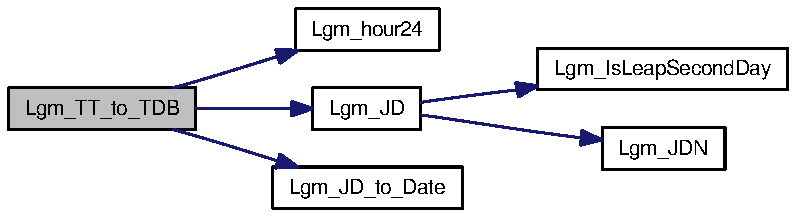
\includegraphics[width=209pt]{_lgm___date_and_time_8c_22d70f08569629bfb06991502e8a2943_cgraph}
\end{center}
\end{figure}


Here is the caller graph for this function:\nopagebreak
\begin{figure}[H]
\begin{center}
\leavevmode
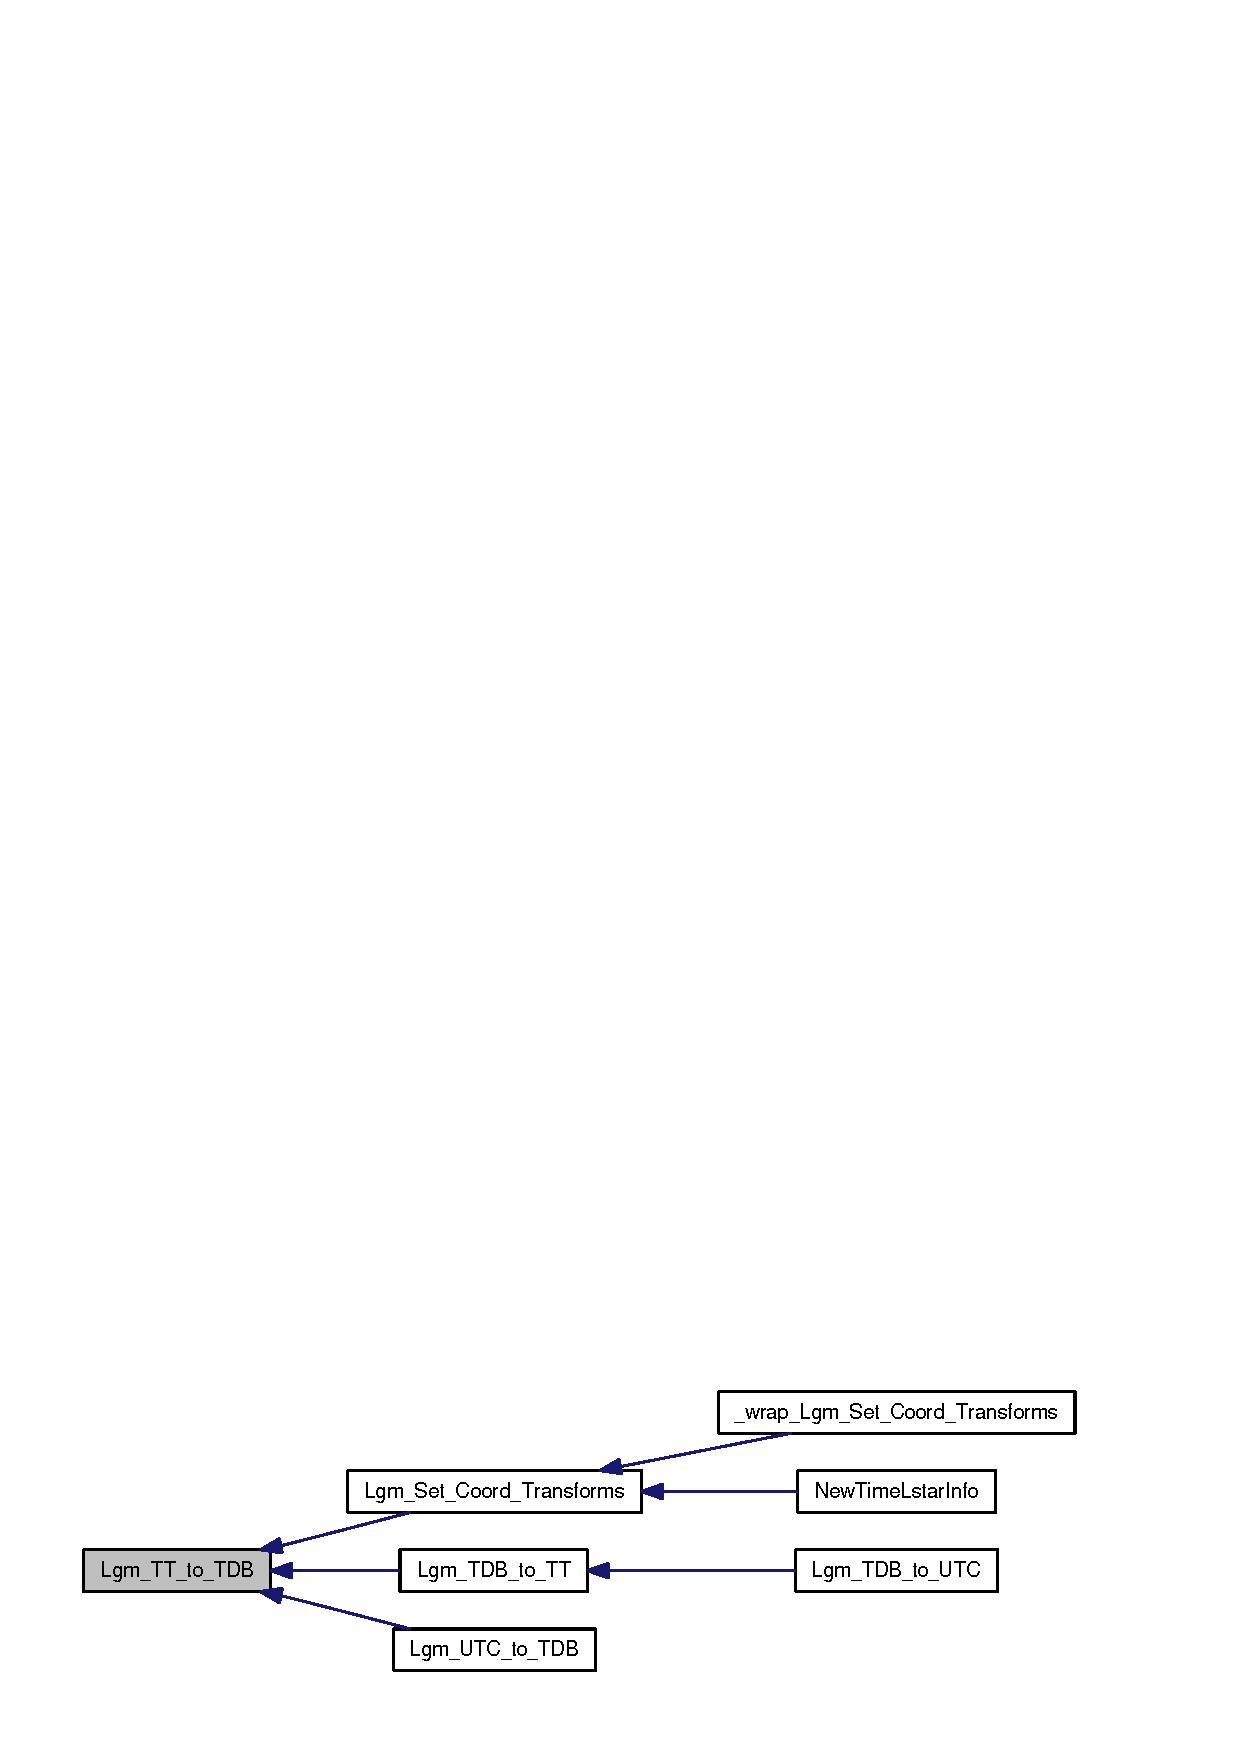
\includegraphics[width=260pt]{_lgm___date_and_time_8c_22d70f08569629bfb06991502e8a2943_icgraph}
\end{center}
\end{figure}
\hypertarget{_lgm___date_and_time_8c_10a71e0d594a09fd5a859d481a7c9dc6}{
\index{Lgm\_\-DateAndTime.c@{Lgm\_\-DateAndTime.c}!Lgm\_\-TT\_\-to\_\-TDB\_\-IAU2006@{Lgm\_\-TT\_\-to\_\-TDB\_\-IAU2006}}
\index{Lgm\_\-TT\_\-to\_\-TDB\_\-IAU2006@{Lgm\_\-TT\_\-to\_\-TDB\_\-IAU2006}!Lgm_DateAndTime.c@{Lgm\_\-DateAndTime.c}}
\subsubsection[{Lgm\_\-TT\_\-to\_\-TDB\_\-IAU2006}]{\setlength{\rightskip}{0pt plus 5cm}void Lgm\_\-TT\_\-to\_\-TDB\_\-IAU2006 ({\bf Lgm\_\-DateTime} $\ast$ {\em TT}, \/  {\bf Lgm\_\-DateTime} $\ast$ {\em TDB}, \/  {\bf Lgm\_\-CTrans} $\ast$ {\em c})}}
\label{_lgm___date_and_time_8c_10a71e0d594a09fd5a859d481a7c9dc6}




Definition at line 665 of file Lgm\_\-DateAndTime.c.

Here is the call graph for this function:\nopagebreak
\begin{figure}[H]
\begin{center}
\leavevmode
\includegraphics[width=231pt]{_lgm___date_and_time_8c_10a71e0d594a09fd5a859d481a7c9dc6_cgraph}
\end{center}
\end{figure}
\hypertarget{_lgm___date_and_time_8c_0d5b5fb558ccb33fe27b2a5452c8e143}{
\index{Lgm\_\-DateAndTime.c@{Lgm\_\-DateAndTime.c}!Lgm\_\-TDB\_\-to\_\-TT@{Lgm\_\-TDB\_\-to\_\-TT}}
\index{Lgm\_\-TDB\_\-to\_\-TT@{Lgm\_\-TDB\_\-to\_\-TT}!Lgm_DateAndTime.c@{Lgm\_\-DateAndTime.c}}
\subsubsection[{Lgm\_\-TDB\_\-to\_\-TT}]{\setlength{\rightskip}{0pt plus 5cm}void Lgm\_\-TDB\_\-to\_\-TT ({\bf Lgm\_\-DateTime} $\ast$ {\em TDB}, \/  {\bf Lgm\_\-DateTime} $\ast$ {\em TT}, \/  {\bf Lgm\_\-CTrans} $\ast$ {\em c})}}
\label{_lgm___date_and_time_8c_0d5b5fb558ccb33fe27b2a5452c8e143}




Definition at line 691 of file Lgm\_\-DateAndTime.c.

Here is the call graph for this function:\nopagebreak
\begin{figure}[H]
\begin{center}
\leavevmode
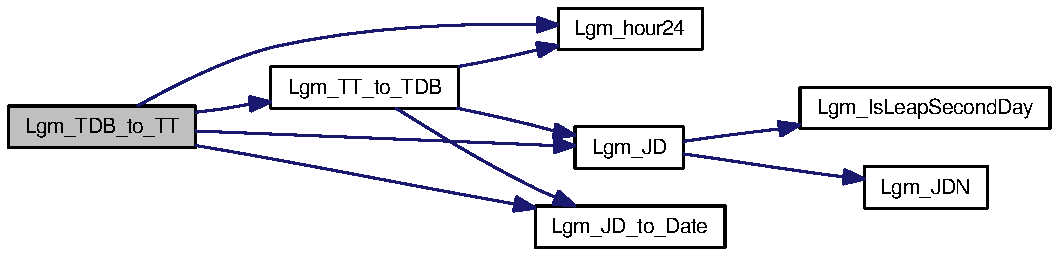
\includegraphics[width=272pt]{_lgm___date_and_time_8c_0d5b5fb558ccb33fe27b2a5452c8e143_cgraph}
\end{center}
\end{figure}


Here is the caller graph for this function:\nopagebreak
\begin{figure}[H]
\begin{center}
\leavevmode
\includegraphics[width=134pt]{_lgm___date_and_time_8c_0d5b5fb558ccb33fe27b2a5452c8e143_icgraph}
\end{center}
\end{figure}
\hypertarget{_lgm___date_and_time_8c_5ee50179c8f841ba7e3377fc23793c37}{
\index{Lgm\_\-DateAndTime.c@{Lgm\_\-DateAndTime.c}!Lgm\_\-UTC\_\-to\_\-TT@{Lgm\_\-UTC\_\-to\_\-TT}}
\index{Lgm\_\-UTC\_\-to\_\-TT@{Lgm\_\-UTC\_\-to\_\-TT}!Lgm_DateAndTime.c@{Lgm\_\-DateAndTime.c}}
\subsubsection[{Lgm\_\-UTC\_\-to\_\-TT}]{\setlength{\rightskip}{0pt plus 5cm}void Lgm\_\-UTC\_\-to\_\-TT ({\bf Lgm\_\-DateTime} $\ast$ {\em UTC}, \/  {\bf Lgm\_\-DateTime} $\ast$ {\em TT}, \/  {\bf Lgm\_\-CTrans} $\ast$ {\em c})}}
\label{_lgm___date_and_time_8c_5ee50179c8f841ba7e3377fc23793c37}




Definition at line 786 of file Lgm\_\-DateAndTime.c.

Here is the call graph for this function:\nopagebreak
\begin{figure}[H]
\begin{center}
\leavevmode
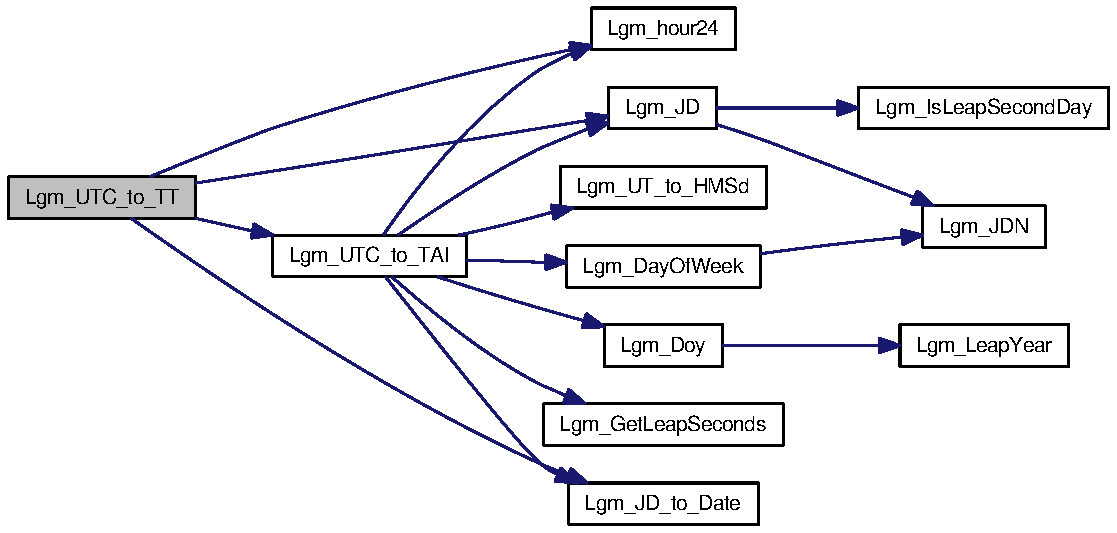
\includegraphics[width=286pt]{_lgm___date_and_time_8c_5ee50179c8f841ba7e3377fc23793c37_cgraph}
\end{center}
\end{figure}


Here is the caller graph for this function:\nopagebreak
\begin{figure}[H]
\begin{center}
\leavevmode
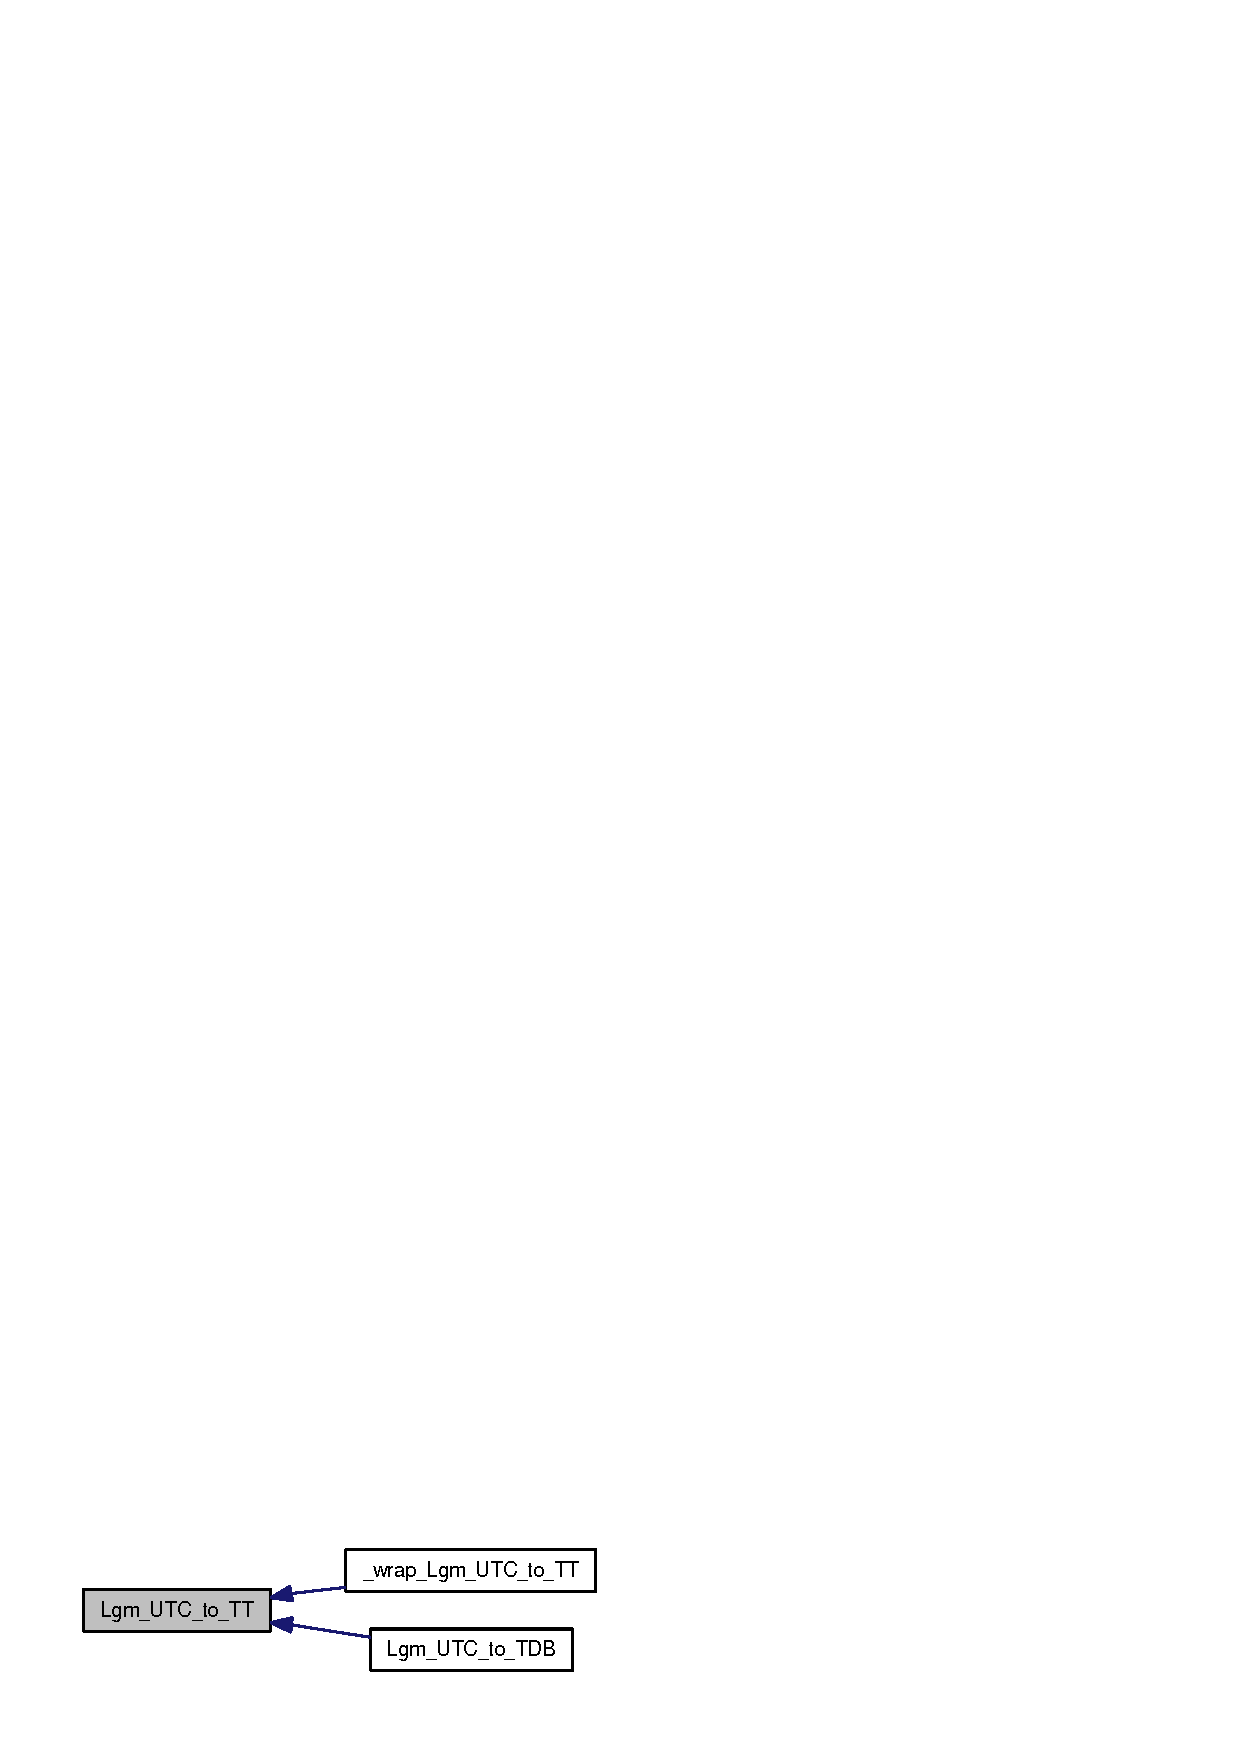
\includegraphics[width=145pt]{_lgm___date_and_time_8c_5ee50179c8f841ba7e3377fc23793c37_icgraph}
\end{center}
\end{figure}
\hypertarget{_lgm___date_and_time_8c_a574b2bf1ef2d8826ecda810565ffc78}{
\index{Lgm\_\-DateAndTime.c@{Lgm\_\-DateAndTime.c}!Lgm\_\-TT\_\-to\_\-UTC@{Lgm\_\-TT\_\-to\_\-UTC}}
\index{Lgm\_\-TT\_\-to\_\-UTC@{Lgm\_\-TT\_\-to\_\-UTC}!Lgm_DateAndTime.c@{Lgm\_\-DateAndTime.c}}
\subsubsection[{Lgm\_\-TT\_\-to\_\-UTC}]{\setlength{\rightskip}{0pt plus 5cm}void Lgm\_\-TT\_\-to\_\-UTC ({\bf Lgm\_\-DateTime} $\ast$ {\em TT}, \/  {\bf Lgm\_\-DateTime} $\ast$ {\em UTC}, \/  {\bf Lgm\_\-CTrans} $\ast$ {\em c})}}
\label{_lgm___date_and_time_8c_a574b2bf1ef2d8826ecda810565ffc78}




Definition at line 810 of file Lgm\_\-DateAndTime.c.

Here is the call graph for this function:\nopagebreak
\begin{figure}[H]
\begin{center}
\leavevmode
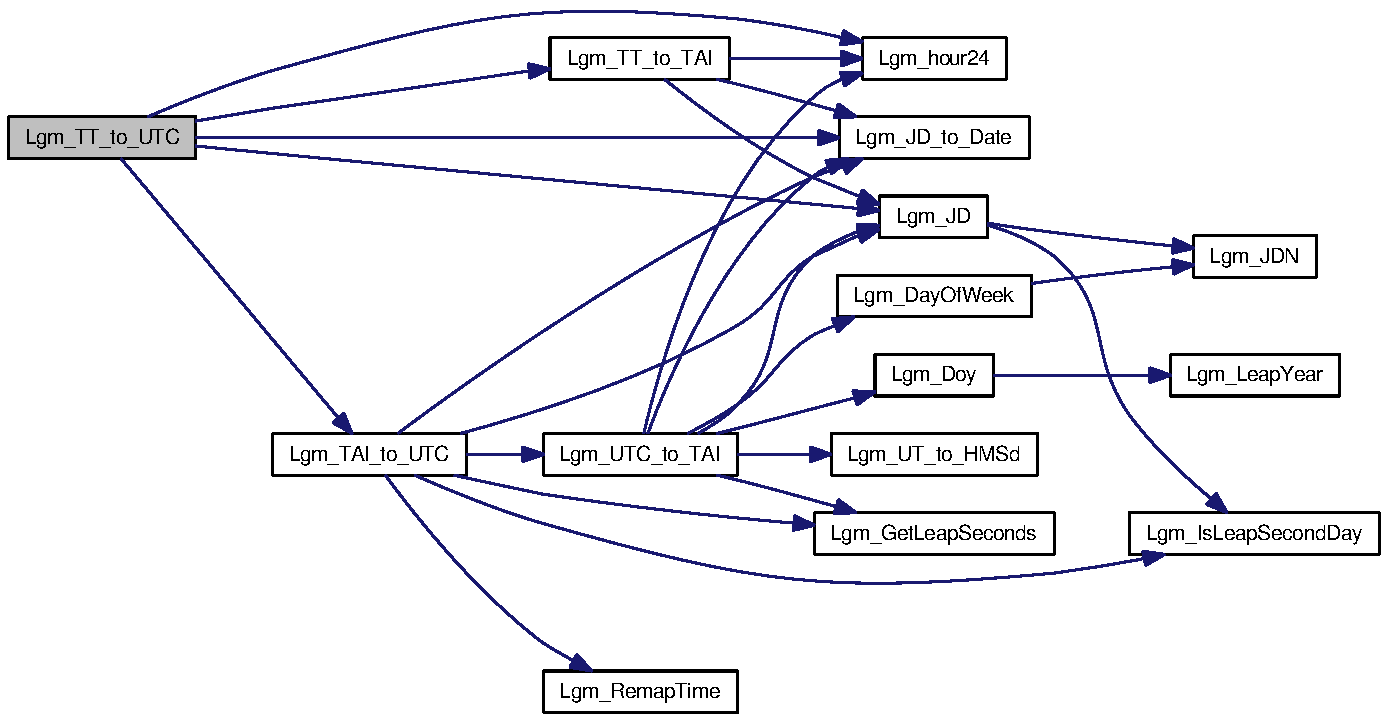
\includegraphics[width=351pt]{_lgm___date_and_time_8c_a574b2bf1ef2d8826ecda810565ffc78_cgraph}
\end{center}
\end{figure}


Here is the caller graph for this function:\nopagebreak
\begin{figure}[H]
\begin{center}
\leavevmode
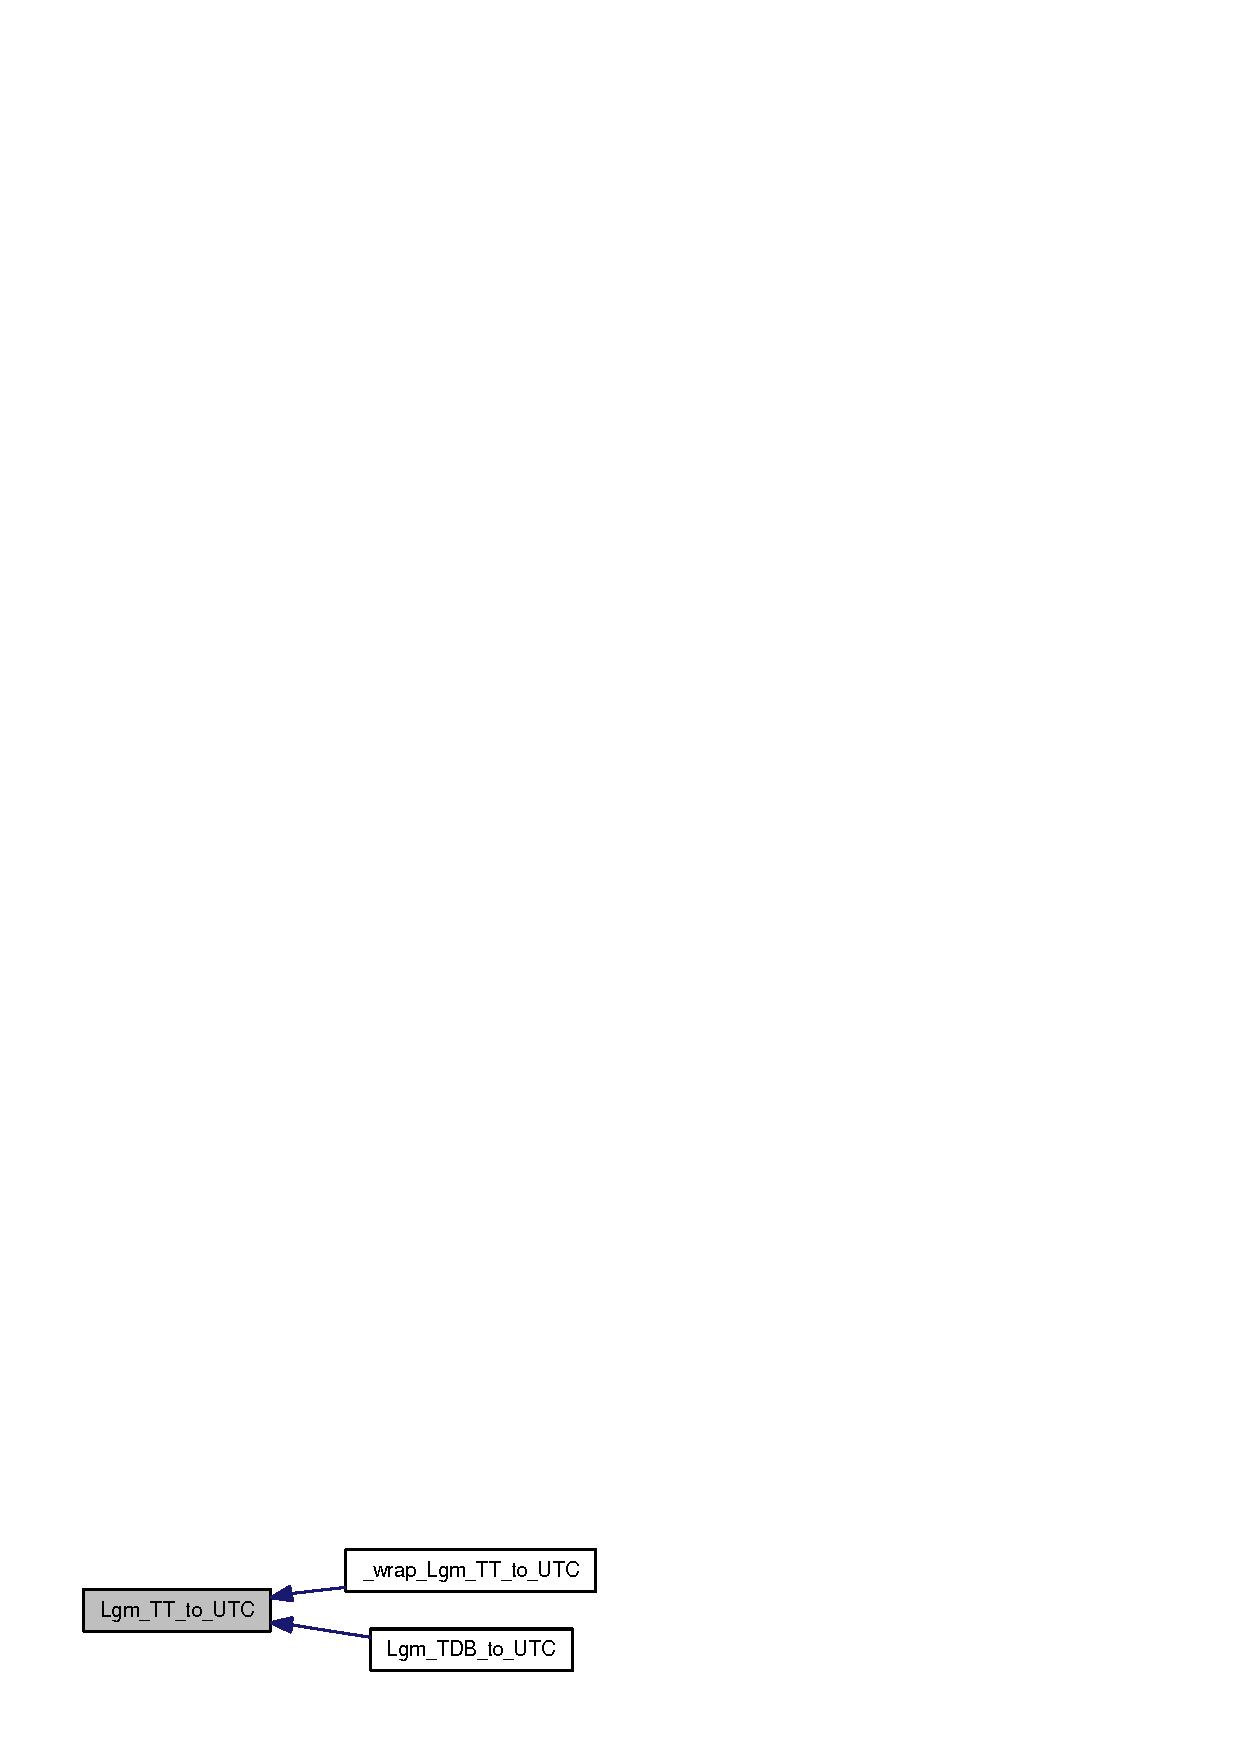
\includegraphics[width=145pt]{_lgm___date_and_time_8c_a574b2bf1ef2d8826ecda810565ffc78_icgraph}
\end{center}
\end{figure}
\hypertarget{_lgm___date_and_time_8c_f30246cdf6676c764baedf2ee8717e9b}{
\index{Lgm\_\-DateAndTime.c@{Lgm\_\-DateAndTime.c}!Lgm\_\-UTC\_\-to\_\-TDB@{Lgm\_\-UTC\_\-to\_\-TDB}}
\index{Lgm\_\-UTC\_\-to\_\-TDB@{Lgm\_\-UTC\_\-to\_\-TDB}!Lgm_DateAndTime.c@{Lgm\_\-DateAndTime.c}}
\subsubsection[{Lgm\_\-UTC\_\-to\_\-TDB}]{\setlength{\rightskip}{0pt plus 5cm}void Lgm\_\-UTC\_\-to\_\-TDB ({\bf Lgm\_\-DateTime} $\ast$ {\em UTC}, \/  {\bf Lgm\_\-DateTime} $\ast$ {\em TDB}, \/  {\bf Lgm\_\-CTrans} $\ast$ {\em c})}}
\label{_lgm___date_and_time_8c_f30246cdf6676c764baedf2ee8717e9b}




Definition at line 837 of file Lgm\_\-DateAndTime.c.

Here is the call graph for this function:\nopagebreak
\begin{figure}[H]
\begin{center}
\leavevmode
\includegraphics[width=353pt]{_lgm___date_and_time_8c_f30246cdf6676c764baedf2ee8717e9b_cgraph}
\end{center}
\end{figure}
\hypertarget{_lgm___date_and_time_8c_04a7c2b17ac1343bdb83bdc8d2204719}{
\index{Lgm\_\-DateAndTime.c@{Lgm\_\-DateAndTime.c}!Lgm\_\-TDB\_\-to\_\-UTC@{Lgm\_\-TDB\_\-to\_\-UTC}}
\index{Lgm\_\-TDB\_\-to\_\-UTC@{Lgm\_\-TDB\_\-to\_\-UTC}!Lgm_DateAndTime.c@{Lgm\_\-DateAndTime.c}}
\subsubsection[{Lgm\_\-TDB\_\-to\_\-UTC}]{\setlength{\rightskip}{0pt plus 5cm}void Lgm\_\-TDB\_\-to\_\-UTC ({\bf Lgm\_\-DateTime} $\ast$ {\em TDB}, \/  {\bf Lgm\_\-DateTime} $\ast$ {\em UTC}, \/  {\bf Lgm\_\-CTrans} $\ast$ {\em c})}}
\label{_lgm___date_and_time_8c_04a7c2b17ac1343bdb83bdc8d2204719}




Definition at line 848 of file Lgm\_\-DateAndTime.c.

Here is the call graph for this function:\nopagebreak
\begin{figure}[H]
\begin{center}
\leavevmode
\includegraphics[width=418pt]{_lgm___date_and_time_8c_04a7c2b17ac1343bdb83bdc8d2204719_cgraph}
\end{center}
\end{figure}
\hypertarget{_lgm___date_and_time_8c_f1fcad21e7b32777e138bb09ca9f8120}{
\index{Lgm\_\-DateAndTime.c@{Lgm\_\-DateAndTime.c}!Lgm\_\-DateTime\_\-Create@{Lgm\_\-DateTime\_\-Create}}
\index{Lgm\_\-DateTime\_\-Create@{Lgm\_\-DateTime\_\-Create}!Lgm_DateAndTime.c@{Lgm\_\-DateAndTime.c}}
\subsubsection[{Lgm\_\-DateTime\_\-Create}]{\setlength{\rightskip}{0pt plus 5cm}{\bf Lgm\_\-DateTime}$\ast$ Lgm\_\-DateTime\_\-Create (int {\em Year}, \/  int {\em Month}, \/  int {\em Day}, \/  double {\em Time}, \/  int {\em TimeSystem}, \/  {\bf Lgm\_\-CTrans} $\ast$ {\em c})}}
\label{_lgm___date_and_time_8c_f1fcad21e7b32777e138bb09ca9f8120}




Definition at line 868 of file Lgm\_\-DateAndTime.c.

Here is the call graph for this function:\nopagebreak
\begin{figure}[H]
\begin{center}
\leavevmode
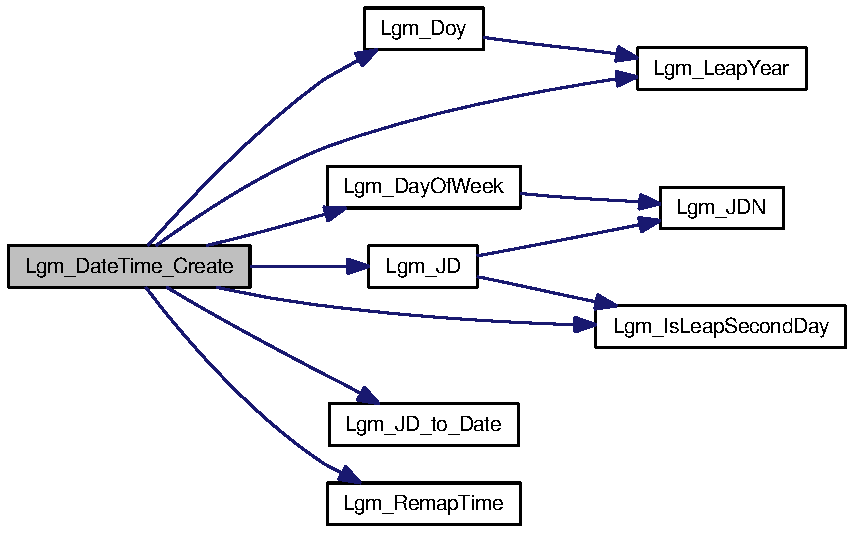
\includegraphics[width=223pt]{_lgm___date_and_time_8c_f1fcad21e7b32777e138bb09ca9f8120_cgraph}
\end{center}
\end{figure}
\hypertarget{_lgm___date_and_time_8c_108f442f417d37e973701a8fae629ba9}{
\index{Lgm\_\-DateAndTime.c@{Lgm\_\-DateAndTime.c}!Lgm\_\-Make\_\-UTC@{Lgm\_\-Make\_\-UTC}}
\index{Lgm\_\-Make\_\-UTC@{Lgm\_\-Make\_\-UTC}!Lgm_DateAndTime.c@{Lgm\_\-DateAndTime.c}}
\subsubsection[{Lgm\_\-Make\_\-UTC}]{\setlength{\rightskip}{0pt plus 5cm}int Lgm\_\-Make\_\-UTC (long int {\em Date}, \/  double {\em Time}, \/  {\bf Lgm\_\-DateTime} $\ast$ {\em UTC}, \/  {\bf Lgm\_\-CTrans} $\ast$ {\em c})}}
\label{_lgm___date_and_time_8c_108f442f417d37e973701a8fae629ba9}




Definition at line 907 of file Lgm\_\-DateAndTime.c.

Here is the call graph for this function:\nopagebreak
\begin{figure}[H]
\begin{center}
\leavevmode
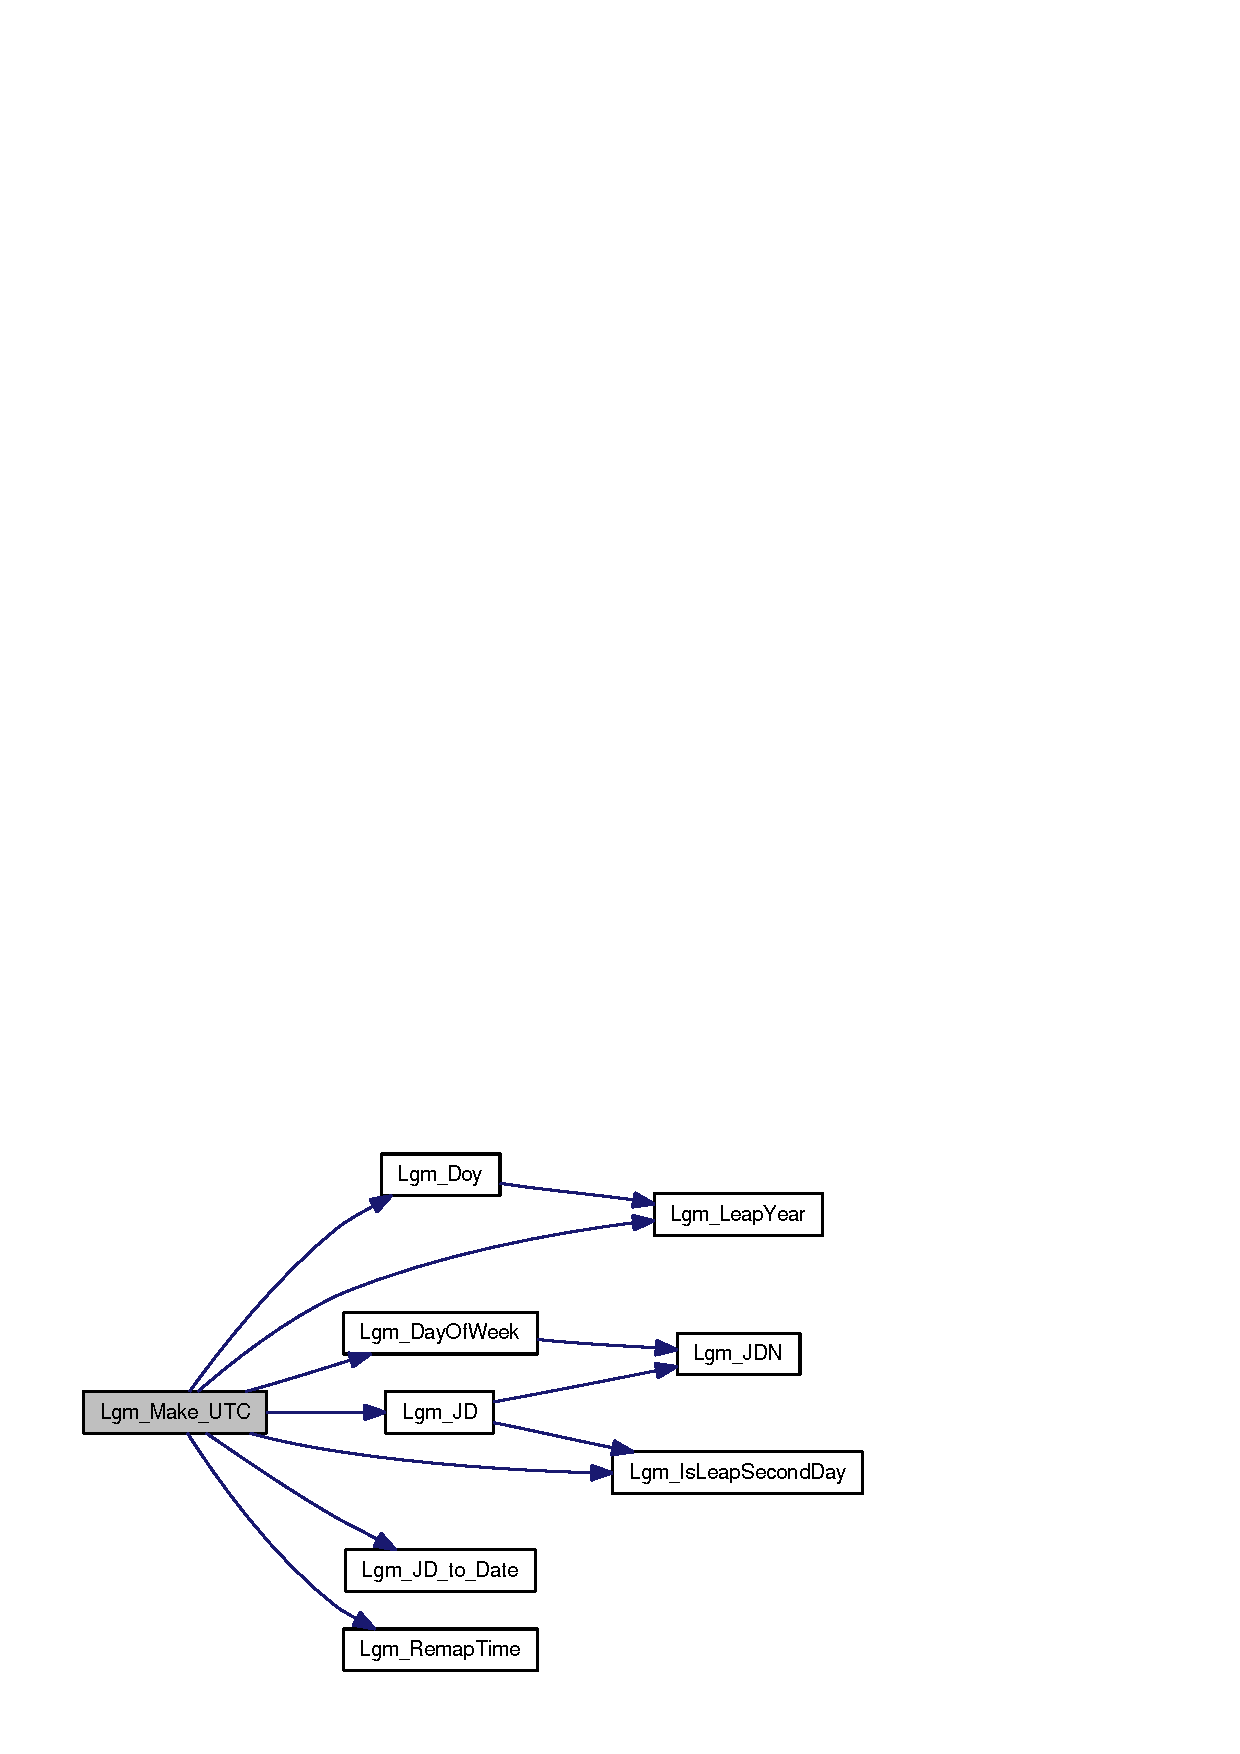
\includegraphics[width=209pt]{_lgm___date_and_time_8c_108f442f417d37e973701a8fae629ba9_cgraph}
\end{center}
\end{figure}
\hypertarget{_lgm___date_and_time_8c_595e9eed10d25d2eb715e7554e83d3f7}{
\index{Lgm\_\-DateAndTime.c@{Lgm\_\-DateAndTime.c}!Lgm\_\-Print\_\-DateTime@{Lgm\_\-Print\_\-DateTime}}
\index{Lgm\_\-Print\_\-DateTime@{Lgm\_\-Print\_\-DateTime}!Lgm_DateAndTime.c@{Lgm\_\-DateAndTime.c}}
\subsubsection[{Lgm\_\-Print\_\-DateTime}]{\setlength{\rightskip}{0pt plus 5cm}void Lgm\_\-Print\_\-DateTime ({\bf Lgm\_\-DateTime} {\em DT}, \/  int {\em Style}, \/  int {\em p})}}
\label{_lgm___date_and_time_8c_595e9eed10d25d2eb715e7554e83d3f7}




Definition at line 951 of file Lgm\_\-DateAndTime.c.

Here is the call graph for this function:\nopagebreak
\begin{figure}[H]
\begin{center}
\leavevmode
\includegraphics[width=153pt]{_lgm___date_and_time_8c_595e9eed10d25d2eb715e7554e83d3f7_cgraph}
\end{center}
\end{figure}
\hypertarget{_lgm___date_and_time_8c_2ec916c82548955c3534f4605ea18c93}{
\index{Lgm\_\-DateAndTime.c@{Lgm\_\-DateAndTime.c}!Lgm\_\-DateTimeToString@{Lgm\_\-DateTimeToString}}
\index{Lgm\_\-DateTimeToString@{Lgm\_\-DateTimeToString}!Lgm_DateAndTime.c@{Lgm\_\-DateAndTime.c}}
\subsubsection[{Lgm\_\-DateTimeToString}]{\setlength{\rightskip}{0pt plus 5cm}void Lgm\_\-DateTimeToString (char $\ast$ {\em Str}, \/  {\bf Lgm\_\-DateTime} {\em DT}, \/  int {\em Style}, \/  int {\em p})}}
\label{_lgm___date_and_time_8c_2ec916c82548955c3534f4605ea18c93}




Definition at line 957 of file Lgm\_\-DateAndTime.c.

Here is the caller graph for this function:\nopagebreak
\begin{figure}[H]
\begin{center}
\leavevmode
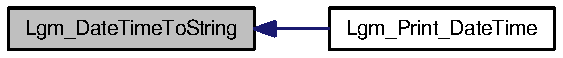
\includegraphics[width=153pt]{_lgm___date_and_time_8c_2ec916c82548955c3534f4605ea18c93_icgraph}
\end{center}
\end{figure}
\hypertarget{_lgm___date_and_time_8c_950485658fca76d3318ee667798563c4}{
\index{Lgm\_\-DateAndTime.c@{Lgm\_\-DateAndTime.c}!Lgm\_\-Print\_\-SimpleTime@{Lgm\_\-Print\_\-SimpleTime}}
\index{Lgm\_\-Print\_\-SimpleTime@{Lgm\_\-Print\_\-SimpleTime}!Lgm_DateAndTime.c@{Lgm\_\-DateAndTime.c}}
\subsubsection[{Lgm\_\-Print\_\-SimpleTime}]{\setlength{\rightskip}{0pt plus 5cm}void Lgm\_\-Print\_\-SimpleTime ({\bf Lgm\_\-DateTime} $\ast$ {\em DT}, \/  int {\em p}, \/  char $\ast$ {\em Str})}}
\label{_lgm___date_and_time_8c_950485658fca76d3318ee667798563c4}




Definition at line 1053 of file Lgm\_\-DateAndTime.c.\hypertarget{_lgm___date_and_time_8c_73a444d73b7a1119517c60f5a070cc9d}{
\index{Lgm\_\-DateAndTime.c@{Lgm\_\-DateAndTime.c}!Lgm\_\-JD@{Lgm\_\-JD}}
\index{Lgm\_\-JD@{Lgm\_\-JD}!Lgm_DateAndTime.c@{Lgm\_\-DateAndTime.c}}
\subsubsection[{Lgm\_\-JD}]{\setlength{\rightskip}{0pt plus 5cm}double Lgm\_\-JD (int {\em Year}, \/  int {\em Month}, \/  int {\em Day}, \/  double {\em Time}, \/  int {\em TimeSystem}, \/  {\bf Lgm\_\-CTrans} $\ast$ {\em c})}}
\label{_lgm___date_and_time_8c_73a444d73b7a1119517c60f5a070cc9d}




Definition at line 1133 of file Lgm\_\-DateAndTime.c.

Here is the call graph for this function:\nopagebreak
\begin{figure}[H]
\begin{center}
\leavevmode
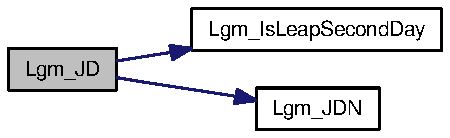
\includegraphics[width=126pt]{_lgm___date_and_time_8c_73a444d73b7a1119517c60f5a070cc9d_cgraph}
\end{center}
\end{figure}


Here is the caller graph for this function:\nopagebreak
\begin{figure}[H]
\begin{center}
\leavevmode
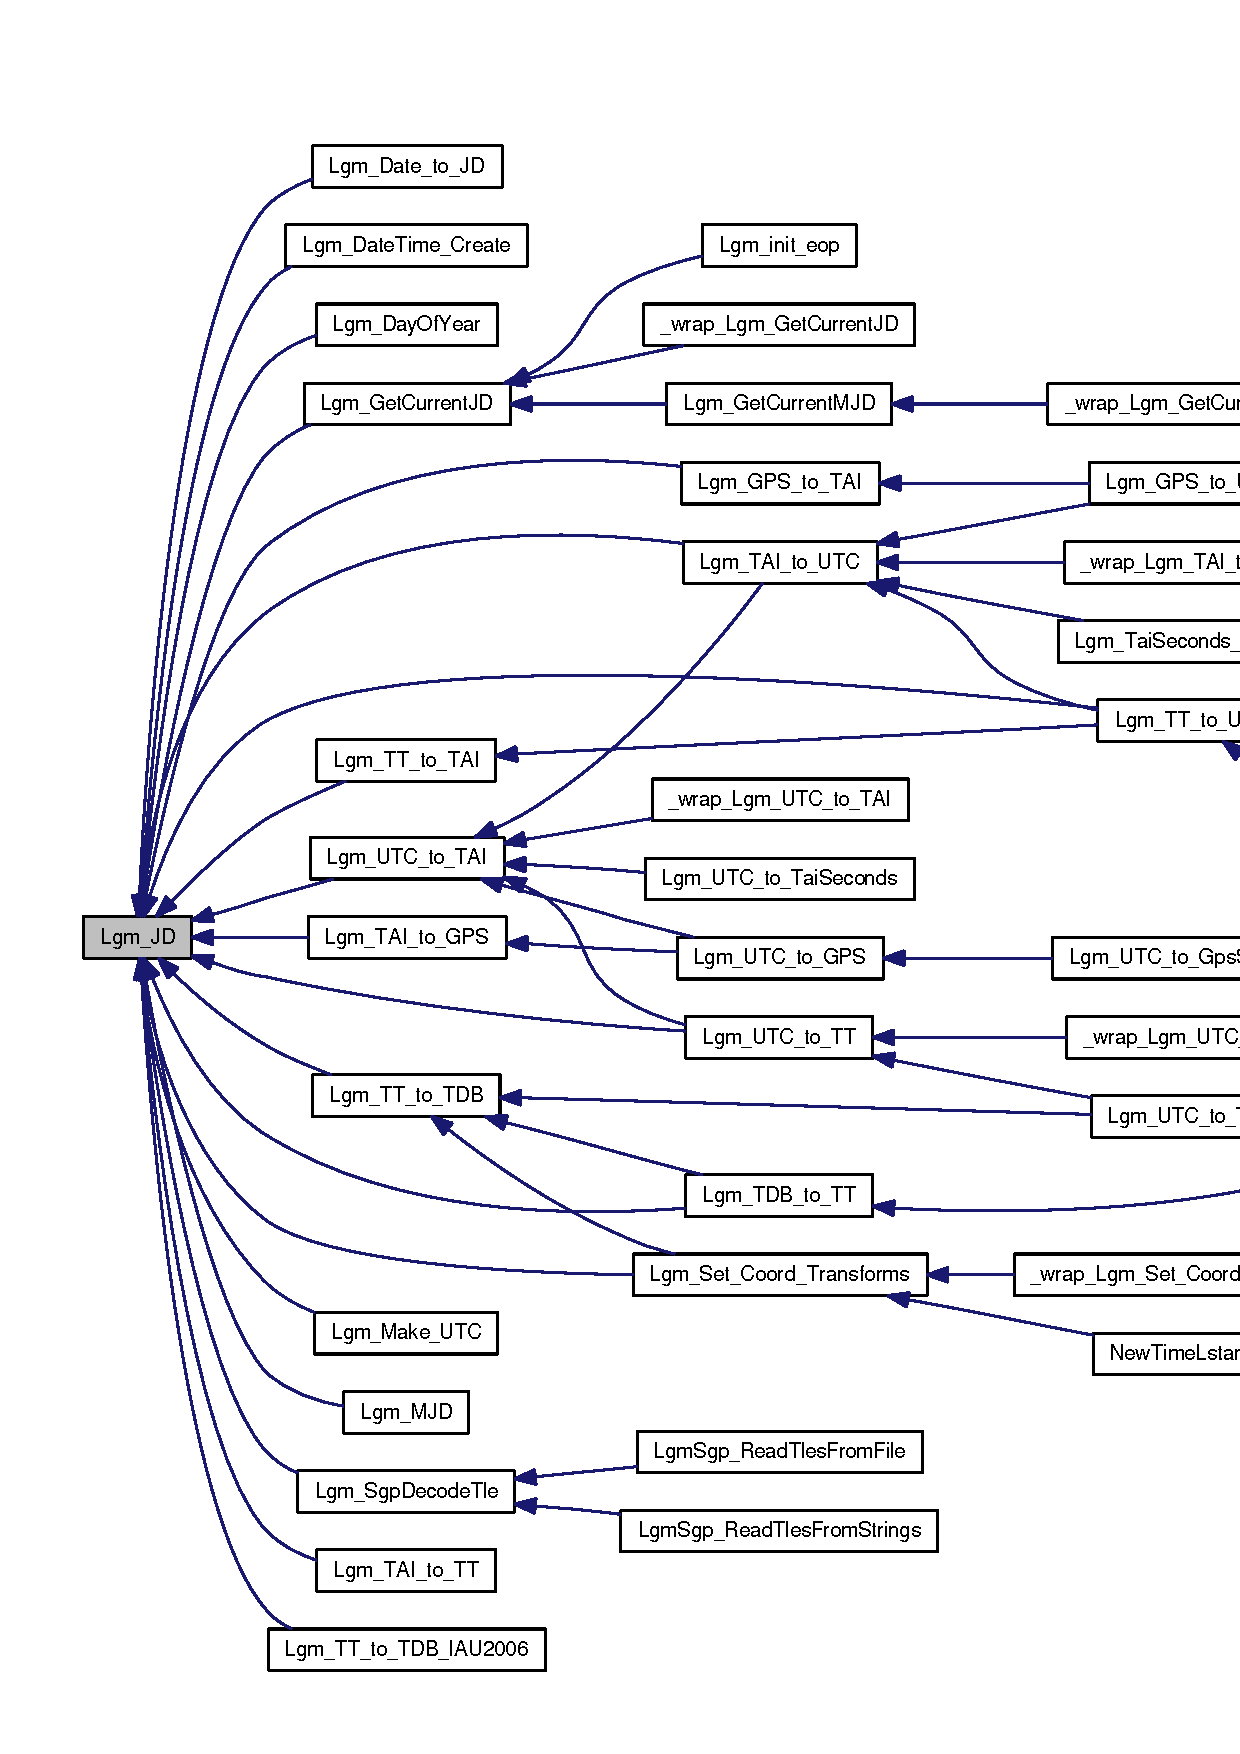
\includegraphics[width=416pt]{_lgm___date_and_time_8c_73a444d73b7a1119517c60f5a070cc9d_icgraph}
\end{center}
\end{figure}
\hypertarget{_lgm___date_and_time_8c_e869fd88ef397bce460b886a6a1b840d}{
\index{Lgm\_\-DateAndTime.c@{Lgm\_\-DateAndTime.c}!Lgm\_\-JDN@{Lgm\_\-JDN}}
\index{Lgm\_\-JDN@{Lgm\_\-JDN}!Lgm_DateAndTime.c@{Lgm\_\-DateAndTime.c}}
\subsubsection[{Lgm\_\-JDN}]{\setlength{\rightskip}{0pt plus 5cm}long int Lgm\_\-JDN (int {\em Year}, \/  int {\em Month}, \/  int {\em Day})}}
\label{_lgm___date_and_time_8c_e869fd88ef397bce460b886a6a1b840d}




Definition at line 1175 of file Lgm\_\-DateAndTime.c.

Here is the caller graph for this function:\nopagebreak
\begin{figure}[H]
\begin{center}
\leavevmode
\includegraphics[width=420pt]{_lgm___date_and_time_8c_e869fd88ef397bce460b886a6a1b840d_icgraph}
\end{center}
\end{figure}
\hypertarget{_lgm___date_and_time_8c_43cca8555131bec5ffeb9d6d39c34b9b}{
\index{Lgm\_\-DateAndTime.c@{Lgm\_\-DateAndTime.c}!Lgm\_\-MJD@{Lgm\_\-MJD}}
\index{Lgm\_\-MJD@{Lgm\_\-MJD}!Lgm_DateAndTime.c@{Lgm\_\-DateAndTime.c}}
\subsubsection[{Lgm\_\-MJD}]{\setlength{\rightskip}{0pt plus 5cm}double Lgm\_\-MJD (int {\em ny}, \/  int {\em nm}, \/  int {\em nd}, \/  double {\em UT}, \/  int {\em TimeSystem}, \/  {\bf Lgm\_\-CTrans} $\ast$ {\em c})}}
\label{_lgm___date_and_time_8c_43cca8555131bec5ffeb9d6d39c34b9b}




Definition at line 1184 of file Lgm\_\-DateAndTime.c.

Here is the call graph for this function:\nopagebreak
\begin{figure}[H]
\begin{center}
\leavevmode
\includegraphics[width=174pt]{_lgm___date_and_time_8c_43cca8555131bec5ffeb9d6d39c34b9b_cgraph}
\end{center}
\end{figure}
\hypertarget{_lgm___date_and_time_8c_ceea9bbfdf0bc68de7a2fe4e406707a3}{
\index{Lgm\_\-DateAndTime.c@{Lgm\_\-DateAndTime.c}!Lgm\_\-Date\_\-to\_\-JD@{Lgm\_\-Date\_\-to\_\-JD}}
\index{Lgm\_\-Date\_\-to\_\-JD@{Lgm\_\-Date\_\-to\_\-JD}!Lgm_DateAndTime.c@{Lgm\_\-DateAndTime.c}}
\subsubsection[{Lgm\_\-Date\_\-to\_\-JD}]{\setlength{\rightskip}{0pt plus 5cm}double Lgm\_\-Date\_\-to\_\-JD (long int {\em Date}, \/  double {\em UT}, \/  {\bf Lgm\_\-CTrans} $\ast$ {\em c})}}
\label{_lgm___date_and_time_8c_ceea9bbfdf0bc68de7a2fe4e406707a3}




Definition at line 1189 of file Lgm\_\-DateAndTime.c.

Here is the call graph for this function:\nopagebreak
\begin{figure}[H]
\begin{center}
\leavevmode
\includegraphics[width=193pt]{_lgm___date_and_time_8c_ceea9bbfdf0bc68de7a2fe4e406707a3_cgraph}
\end{center}
\end{figure}
\hypertarget{_lgm___date_and_time_8c_1808acdcc963d25827db876e77d17b5f}{
\index{Lgm\_\-DateAndTime.c@{Lgm\_\-DateAndTime.c}!Lgm\_\-DayOfYear@{Lgm\_\-DayOfYear}}
\index{Lgm\_\-DayOfYear@{Lgm\_\-DayOfYear}!Lgm_DateAndTime.c@{Lgm\_\-DateAndTime.c}}
\subsubsection[{Lgm\_\-DayOfYear}]{\setlength{\rightskip}{0pt plus 5cm}int Lgm\_\-DayOfYear (int {\em year}, \/  int {\em month}, \/  int {\em day}, \/  {\bf Lgm\_\-CTrans} $\ast$ {\em c})}}
\label{_lgm___date_and_time_8c_1808acdcc963d25827db876e77d17b5f}




Definition at line 1198 of file Lgm\_\-DateAndTime.c.

Here is the call graph for this function:\nopagebreak
\begin{figure}[H]
\begin{center}
\leavevmode
\includegraphics[width=188pt]{_lgm___date_and_time_8c_1808acdcc963d25827db876e77d17b5f_cgraph}
\end{center}
\end{figure}
\hypertarget{_lgm___date_and_time_8c_38f91ae9f05bbcd134091cea464ee003}{
\index{Lgm\_\-DateAndTime.c@{Lgm\_\-DateAndTime.c}!Lgm\_\-DayOfWeek@{Lgm\_\-DayOfWeek}}
\index{Lgm\_\-DayOfWeek@{Lgm\_\-DayOfWeek}!Lgm_DateAndTime.c@{Lgm\_\-DateAndTime.c}}
\subsubsection[{Lgm\_\-DayOfWeek}]{\setlength{\rightskip}{0pt plus 5cm}int Lgm\_\-DayOfWeek (int {\em Year}, \/  int {\em Month}, \/  int {\em Day}, \/  char $\ast$ {\em dowstr})}}
\label{_lgm___date_and_time_8c_38f91ae9f05bbcd134091cea464ee003}




Definition at line 1205 of file Lgm\_\-DateAndTime.c.

Here is the call graph for this function:\nopagebreak
\begin{figure}[H]
\begin{center}
\leavevmode
\includegraphics[width=117pt]{_lgm___date_and_time_8c_38f91ae9f05bbcd134091cea464ee003_cgraph}
\end{center}
\end{figure}


Here is the caller graph for this function:\nopagebreak
\begin{figure}[H]
\begin{center}
\leavevmode
\includegraphics[width=420pt]{_lgm___date_and_time_8c_38f91ae9f05bbcd134091cea464ee003_icgraph}
\end{center}
\end{figure}
\hypertarget{_lgm___date_and_time_8c_55fe73d488049143abdf53aed109af07}{
\index{Lgm\_\-DateAndTime.c@{Lgm\_\-DateAndTime.c}!Lgm\_\-Doy@{Lgm\_\-Doy}}
\index{Lgm\_\-Doy@{Lgm\_\-Doy}!Lgm_DateAndTime.c@{Lgm\_\-DateAndTime.c}}
\subsubsection[{Lgm\_\-Doy}]{\setlength{\rightskip}{0pt plus 5cm}int Lgm\_\-Doy (long int {\em date}, \/  int $\ast$ {\em YY}, \/  int $\ast$ {\em MM}, \/  int $\ast$ {\em DD}, \/  int $\ast$ {\em DOY})}}
\label{_lgm___date_and_time_8c_55fe73d488049143abdf53aed109af07}




Definition at line 1242 of file Lgm\_\-DateAndTime.c.

Here is the call graph for this function:\nopagebreak
\begin{figure}[H]
\begin{center}
\leavevmode
\includegraphics[width=110pt]{_lgm___date_and_time_8c_55fe73d488049143abdf53aed109af07_cgraph}
\end{center}
\end{figure}


Here is the caller graph for this function:\nopagebreak
\begin{figure}[H]
\begin{center}
\leavevmode
\includegraphics[width=414pt]{_lgm___date_and_time_8c_55fe73d488049143abdf53aed109af07_icgraph}
\end{center}
\end{figure}
\hypertarget{_lgm___date_and_time_8c_b9dde7da7103f227bc6b698bed55e9ab}{
\index{Lgm\_\-DateAndTime.c@{Lgm\_\-DateAndTime.c}!Lgm\_\-IsValidDate@{Lgm\_\-IsValidDate}}
\index{Lgm\_\-IsValidDate@{Lgm\_\-IsValidDate}!Lgm_DateAndTime.c@{Lgm\_\-DateAndTime.c}}
\subsubsection[{Lgm\_\-IsValidDate}]{\setlength{\rightskip}{0pt plus 5cm}int Lgm\_\-IsValidDate (long int {\em Date})}}
\label{_lgm___date_and_time_8c_b9dde7da7103f227bc6b698bed55e9ab}




Definition at line 1298 of file Lgm\_\-DateAndTime.c.

Here is the call graph for this function:\nopagebreak
\begin{figure}[H]
\begin{center}
\leavevmode
\includegraphics[width=173pt]{_lgm___date_and_time_8c_b9dde7da7103f227bc6b698bed55e9ab_cgraph}
\end{center}
\end{figure}


Here is the caller graph for this function:\nopagebreak
\begin{figure}[H]
\begin{center}
\leavevmode
\includegraphics[width=146pt]{_lgm___date_and_time_8c_b9dde7da7103f227bc6b698bed55e9ab_icgraph}
\end{center}
\end{figure}
\hypertarget{_lgm___date_and_time_8c_af81b2f637efd027fd4fb425f16dd027}{
\index{Lgm\_\-DateAndTime.c@{Lgm\_\-DateAndTime.c}!Lgm\_\-RemapTime@{Lgm\_\-RemapTime}}
\index{Lgm\_\-RemapTime@{Lgm\_\-RemapTime}!Lgm_DateAndTime.c@{Lgm\_\-DateAndTime.c}}
\subsubsection[{Lgm\_\-RemapTime}]{\setlength{\rightskip}{0pt plus 5cm}double Lgm\_\-RemapTime (double {\em Time}, \/  double {\em SecondsInADay})}}
\label{_lgm___date_and_time_8c_af81b2f637efd027fd4fb425f16dd027}




Definition at line 1325 of file Lgm\_\-DateAndTime.c.

Here is the caller graph for this function:\nopagebreak
\begin{figure}[H]
\begin{center}
\leavevmode
\includegraphics[width=313pt]{_lgm___date_and_time_8c_af81b2f637efd027fd4fb425f16dd027_icgraph}
\end{center}
\end{figure}
\hypertarget{_lgm___date_and_time_8c_70d002da98009a23c04a5ba8a934caeb}{
\index{Lgm\_\-DateAndTime.c@{Lgm\_\-DateAndTime.c}!Lgm\_\-UTC\_\-to\_\-TDBSeconds@{Lgm\_\-UTC\_\-to\_\-TDBSeconds}}
\index{Lgm\_\-UTC\_\-to\_\-TDBSeconds@{Lgm\_\-UTC\_\-to\_\-TDBSeconds}!Lgm_DateAndTime.c@{Lgm\_\-DateAndTime.c}}
\subsubsection[{Lgm\_\-UTC\_\-to\_\-TDBSeconds}]{\setlength{\rightskip}{0pt plus 5cm}double Lgm\_\-UTC\_\-to\_\-TDBSeconds ({\bf Lgm\_\-DateTime} $\ast$ {\em UTC}, \/  {\bf Lgm\_\-CTrans} $\ast$ {\em c})}}
\label{_lgm___date_and_time_8c_70d002da98009a23c04a5ba8a934caeb}




Definition at line 1347 of file Lgm\_\-DateAndTime.c.

Here is the call graph for this function:\nopagebreak
\begin{figure}[H]
\begin{center}
\leavevmode
\includegraphics[width=239pt]{_lgm___date_and_time_8c_70d002da98009a23c04a5ba8a934caeb_cgraph}
\end{center}
\end{figure}
\hypertarget{_lgm___date_and_time_8c_07aa79aa96c76993e5770b7a5967f663}{
\index{Lgm\_\-DateAndTime.c@{Lgm\_\-DateAndTime.c}!Lgm\_\-TDBSecSinceJ2000@{Lgm\_\-TDBSecSinceJ2000}}
\index{Lgm\_\-TDBSecSinceJ2000@{Lgm\_\-TDBSecSinceJ2000}!Lgm_DateAndTime.c@{Lgm\_\-DateAndTime.c}}
\subsubsection[{Lgm\_\-TDBSecSinceJ2000}]{\setlength{\rightskip}{0pt plus 5cm}double Lgm\_\-TDBSecSinceJ2000 ({\bf Lgm\_\-DateTime} $\ast$ {\em UTC}, \/  {\bf Lgm\_\-CTrans} $\ast$ {\em c})}}
\label{_lgm___date_and_time_8c_07aa79aa96c76993e5770b7a5967f663}




Definition at line 1350 of file Lgm\_\-DateAndTime.c.

Here is the call graph for this function:\nopagebreak
\begin{figure}[H]
\begin{center}
\leavevmode
\includegraphics[width=153pt]{_lgm___date_and_time_8c_07aa79aa96c76993e5770b7a5967f663_cgraph}
\end{center}
\end{figure}


Here is the caller graph for this function:\nopagebreak
\begin{figure}[H]
\begin{center}
\leavevmode
\includegraphics[width=172pt]{_lgm___date_and_time_8c_07aa79aa96c76993e5770b7a5967f663_icgraph}
\end{center}
\end{figure}
